\documentclass[]{article}

%These tell TeX which packages to use.
\usepackage{array,epsfig}
\usepackage{amsmath}
\usepackage{amsfonts}
\usepackage{amssymb}
\usepackage{amsxtra}
\usepackage{amsthm}
\usepackage{mathrsfs}
\usepackage{color}
\usepackage{graphicx}
\usepackage{xcolor}
\usepackage{float}
\usepackage{framed}
\usepackage{empheq}
\usepackage[utf8]{inputenc}
\usepackage{fancyhdr}
\raggedbottom


%Here I define some theorem styles and shortcut commands for symbols I use often
\theoremstyle{definition}
\newtheorem{defn}{Definition}
\newtheorem{thm}{Theorem}
\newtheorem{cor}{Corollary}
\newtheorem*{rmk}{Remark}
\newtheorem{lem}{Lemma}
\newtheorem*{joke}{Joke}
\newtheorem{ex}{Example}
\newtheorem*{soln}{Solution}
\newtheorem{prop}{Proposition}

\newcommand{\lra}{\longrightarrow}
\newcommand{\ra}{\rightarrow}
\newcommand{\surj}{\twoheadrightarrow}
\newcommand{\graph}{\mathrm{graph}}
\newcommand{\bb}[1]{\mathbb{#1}}
\newcommand{\Z}{\bb{Z}}
\newcommand{\Q}{\bb{Q}}
\newcommand{\R}{\bb{R}}
\newcommand{\C}{\bb{C}}
\newcommand{\N}{\bb{N}}
\newcommand{\M}{\mathbf{M}}
\newcommand{\m}{\mathbf{m}}
\newcommand{\MM}{\mathscr{M}}
\newcommand{\HH}{\mathscr{H}}
\newcommand{\Om}{\Omega}
\newcommand{\Ho}{\in\HH(\Om)}
\newcommand{\bd}{\partial}
\newcommand{\del}{\partial}
\newcommand{\bardel}{\overline\partial}
\newcommand{\textdf}[1]{\textbf{\textsf{#1}}\index{#1}}
\newcommand{\img}{\mathrm{img}}
\newcommand{\ip}[2]{\left\langle{#1},{#2}\right\rangle}
\newcommand{\inter}[1]{\mathrm{int}{#1}}
\newcommand{\exter}[1]{\mathrm{ext}{#1}}
\newcommand{\cl}[1]{\mathrm{cl}{#1}}
\newcommand{\ds}{\displaystyle}
\newcommand{\vol}{\mathrm{vol}}
\newcommand{\cnt}{\mathrm{ct}}
\newcommand{\osc}{\mathrm{osc}}
\newcommand{\LL}{\mathbf{L}}
\newcommand{\UU}{\mathbf{U}}
\newcommand{\support}{\mathrm{support}}
\newcommand{\AND}{\;\wedge\;}
\newcommand{\OR}{\;\vee\;}
\newcommand{\Oset}{\varnothing}
\newcommand{\st}{\ni}
\newcommand{\wh}{\widehat}

%Pagination stuff.
\setlength{\topmargin}{-.3 in}
\setlength{\oddsidemargin}{0in}
\setlength{\evensidemargin}{0in}
\setlength{\textheight}{9.in}
\setlength{\textwidth}{6.5in}
\pagestyle{empty}
\pagestyle{fancy}
\fancyhf{}
\fancyfoot[C]{\thepage}
\renewcommand{\headrulewidth}{0pt}
\pagenumbering{arabic}

\begin{document}
\begin{center}
{\textbf{\Large AE601 Mathematical Methods in Aerospace Engineering}}\\

\normalsize{Submitted by Ramesh M (SC23M061)}\\
\end{center}

\vspace{0.2 cm}

\begin{enumerate}
%1a starts
\item 
Solve the one-dimensional heat equation
\[
\frac{\partial u}{\partial t} = \alpha \frac{\partial^2 u}{\partial x^2}, \quad 0 < x < L, \, t > 0
\]
in a finite domain for the following initial and boundary conditions:\\
\textbf{(a)}\quad
\begin{align*}
u(x,0) &= U, \quad 0 < x < L \\
u(0,t) &= 0 \\
u(L,t) &= 0
\end{align*}
where \(U\) is a constant. Find the location of the maximum temperature for \(t > 0\).\\
\\
\emph{\textbf{Solution:}}\\
We have two homogeneous boundary conditions, so using method of separation of variables to solve the problem:
\[
u(x,t) = X(x)\cdot T(t)
\]
Substituting this in the one dimensional heat equation we get,
\[
X(x) = C_1cos(kx) + C_2sin(kx)
\]
\[
T(x) = C_3e^{(-\alpha\cdot k^2\cdot t)}
\]
Solving for $C_1$, $C_2$, $C_3$ and $k$ by applying the Boundary conditions,
\[
k = \frac{n\pi}{L}
\]
\[
\boxed{
B_n = \frac{2 U}{\pi}(1 - (-1)^n)
}
\]
\[
\boxed{
u(x,t) = \sum_{n=1}^{\infty} \frac{2 U}{\pi}(1 - (-1)^n)\cdot e^{(-\alpha\cdot (\frac{n\pi}{2})^2\cdot t)}\cdot sin(\frac{n\pi x}{L})
}
\]

The values are assumed for plotting, \\
Thermal diffusivity, $\alpha = 1.115 \times 10^{-3}\, \text{m}^2/\text{s}$ \\
Initial temperature, $U = 50\, \text{K}$ \\
Length of the domain, $L = 1\, \text{m}$ \\
The plot is shown below:\\
\begin{figure}[htbp]
    \centering
    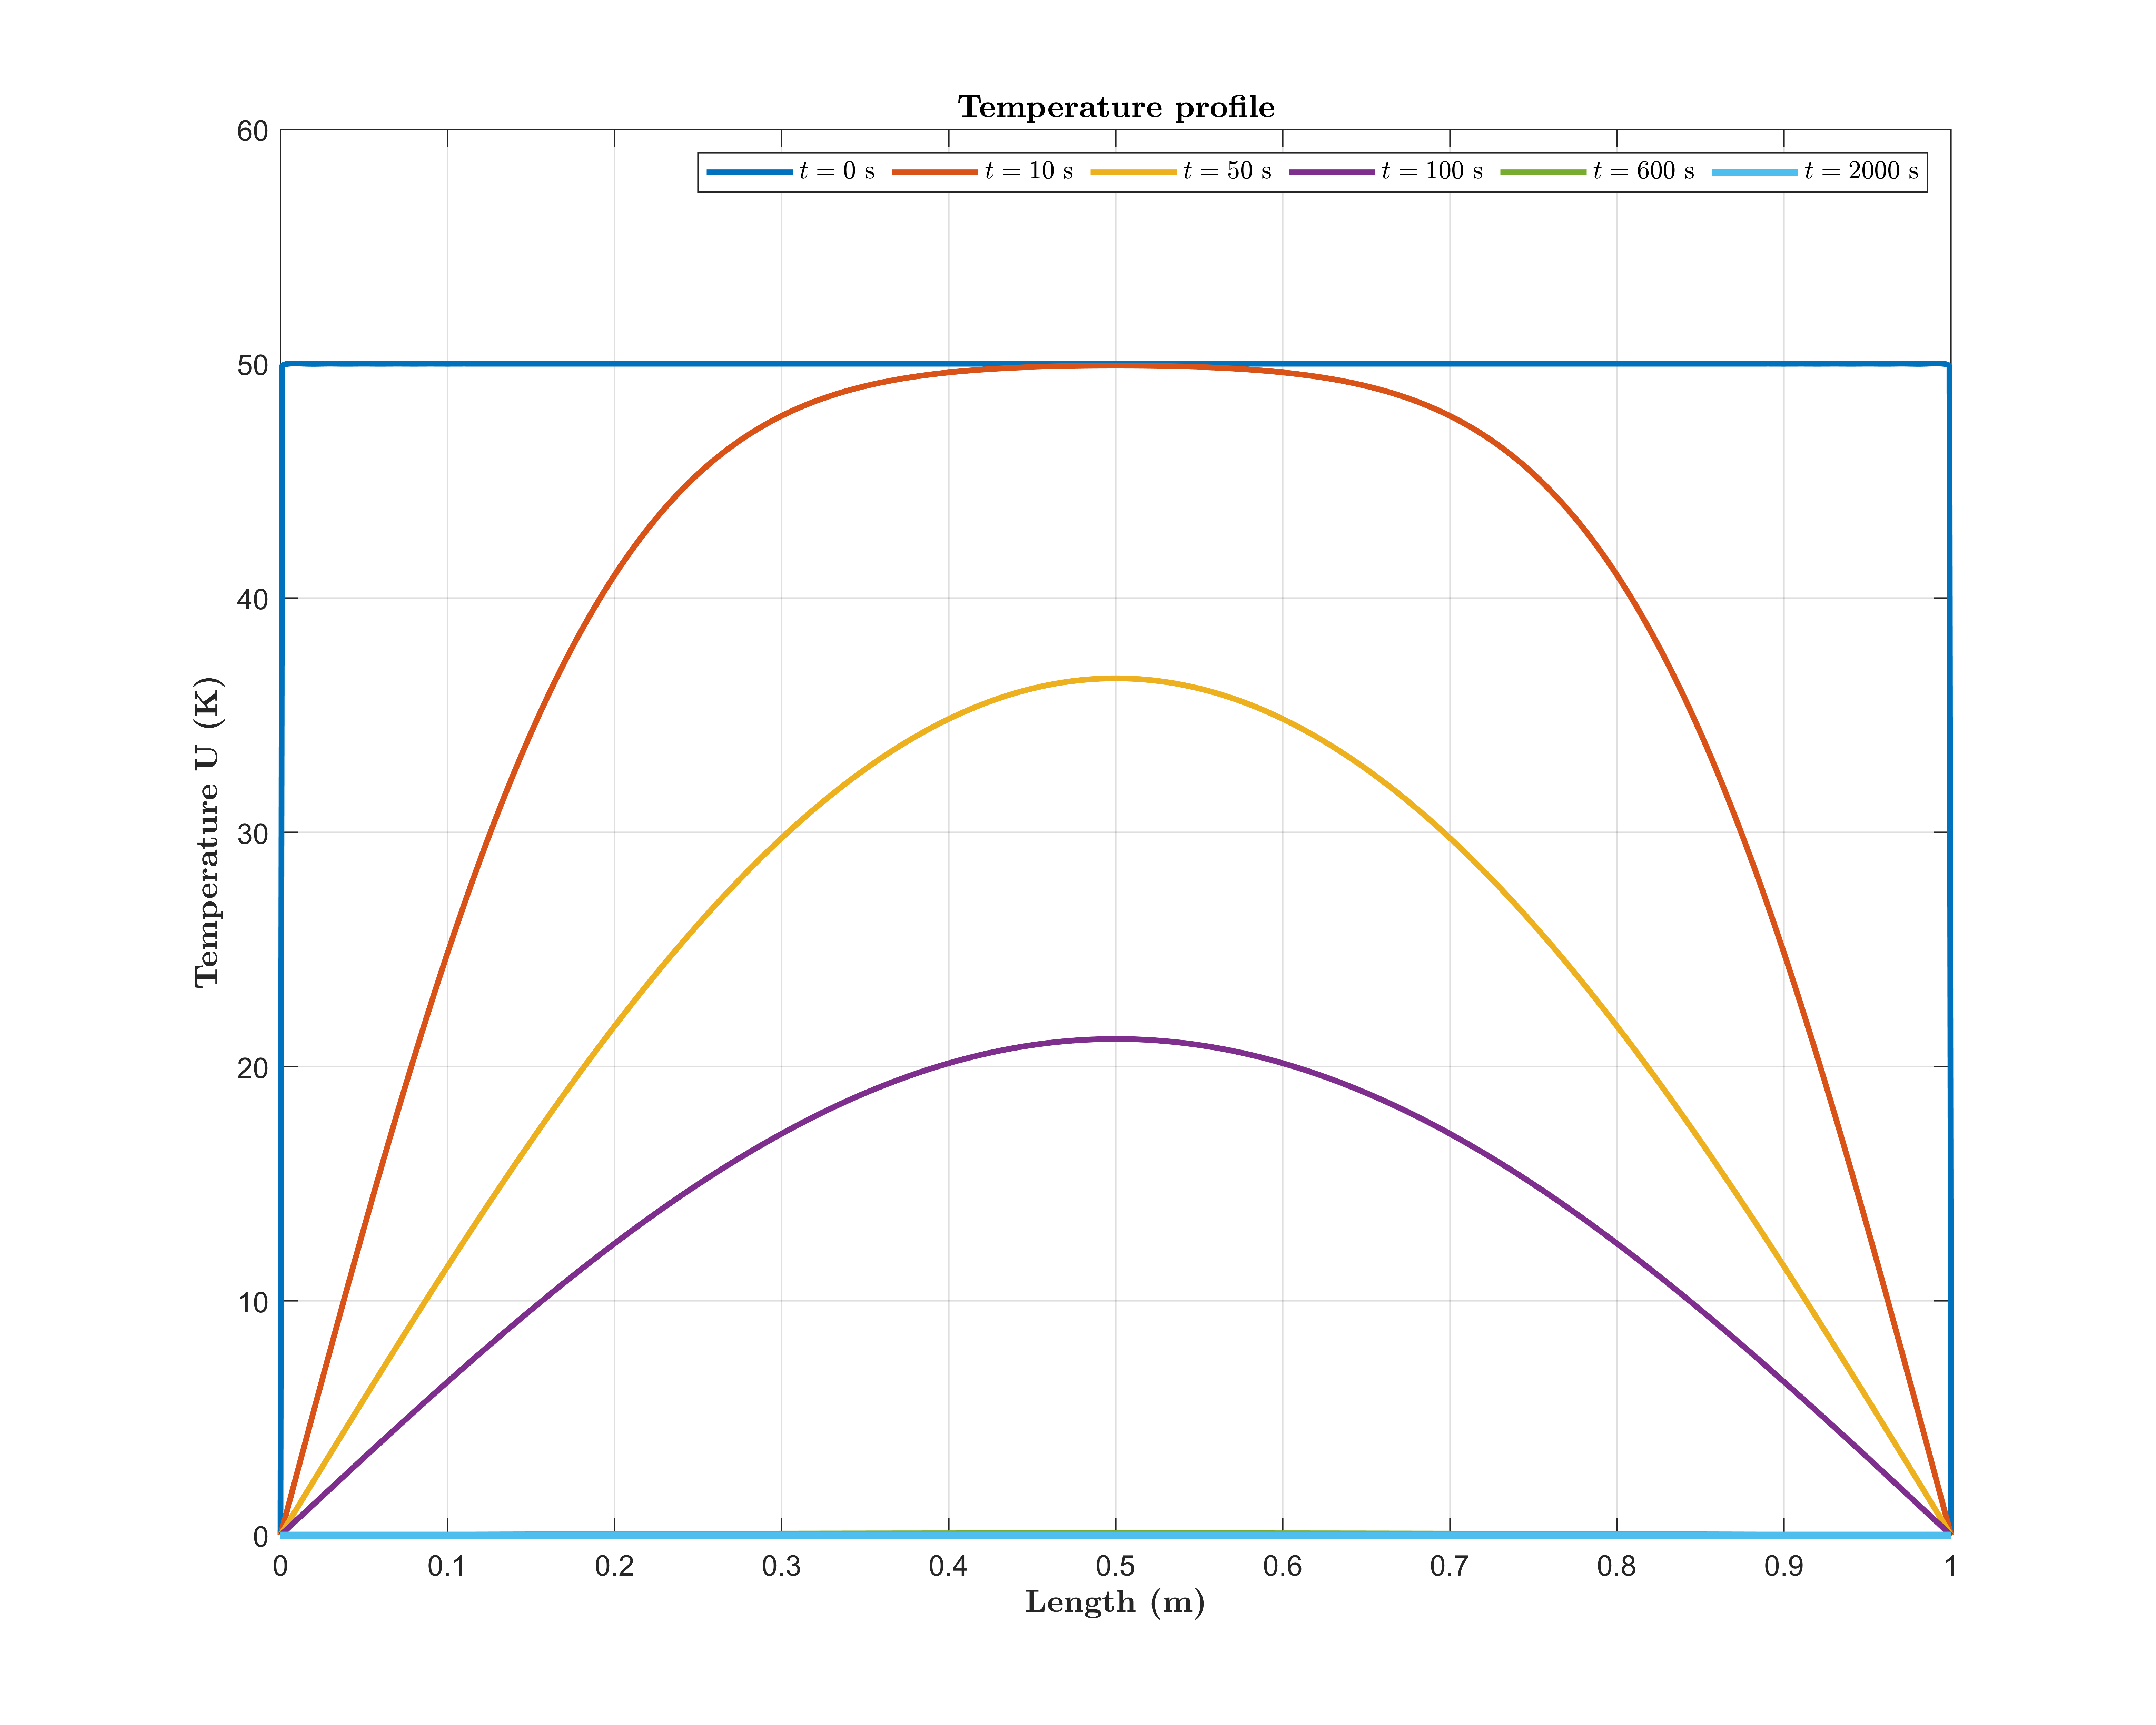
\includegraphics[width=0.8\textwidth]{Images/Problem_1_a.png}
\end{figure}\\
%1a ends
\pagebreak

%%%%%%%%%%%%%%%%%%%%%%%%%%%%%%%%%%%%%%%%%%%%%%%%%%%%%%%%%%%%%%%%%%
%1b starts
\textbf{(b)}\quad
\begin{align*}
u(x,0) &= \begin{cases}
x, & 0 < x \leq \frac{L}{2} \\
L - x, & \frac{L}{2} < x < L
\end{cases} \\
u(0,t) &= 0 \\
u(L,t) &= 0 \\
\end{align*}
\emph{\textbf{Solution:}}\\
Following the same procedure as $a$, $B_n$ can be calculated,
\[
B_n = \frac{4L}{(n\pi)^2} \cdot \sin\left(\frac{n\pi}{2}\right)
\]
The total solution will be,
\[
\boxed{
u(x,t) = \sum_{n=1}^{\infty} \frac{4L}{(n\pi)^2} \cdot \sin\left(\frac{n\pi}{2}\right) \cdot e^{-\alpha \cdot \left(\frac{n\pi}{2}\right)^2 \cdot t} \cdot \sin\left(\frac{n\pi x}{L}\right)
}
\]
The values are assumed for plotting, \\
Thermal diffusivity, $\alpha = 1.115 \times 10^{-3}\, \text{m}^2/\text{s}$ \\
Length of the domain, $L = 1\, \text{m}$ \\
The plot is shown below:\\
\begin{figure}[htbp]
    \centering
    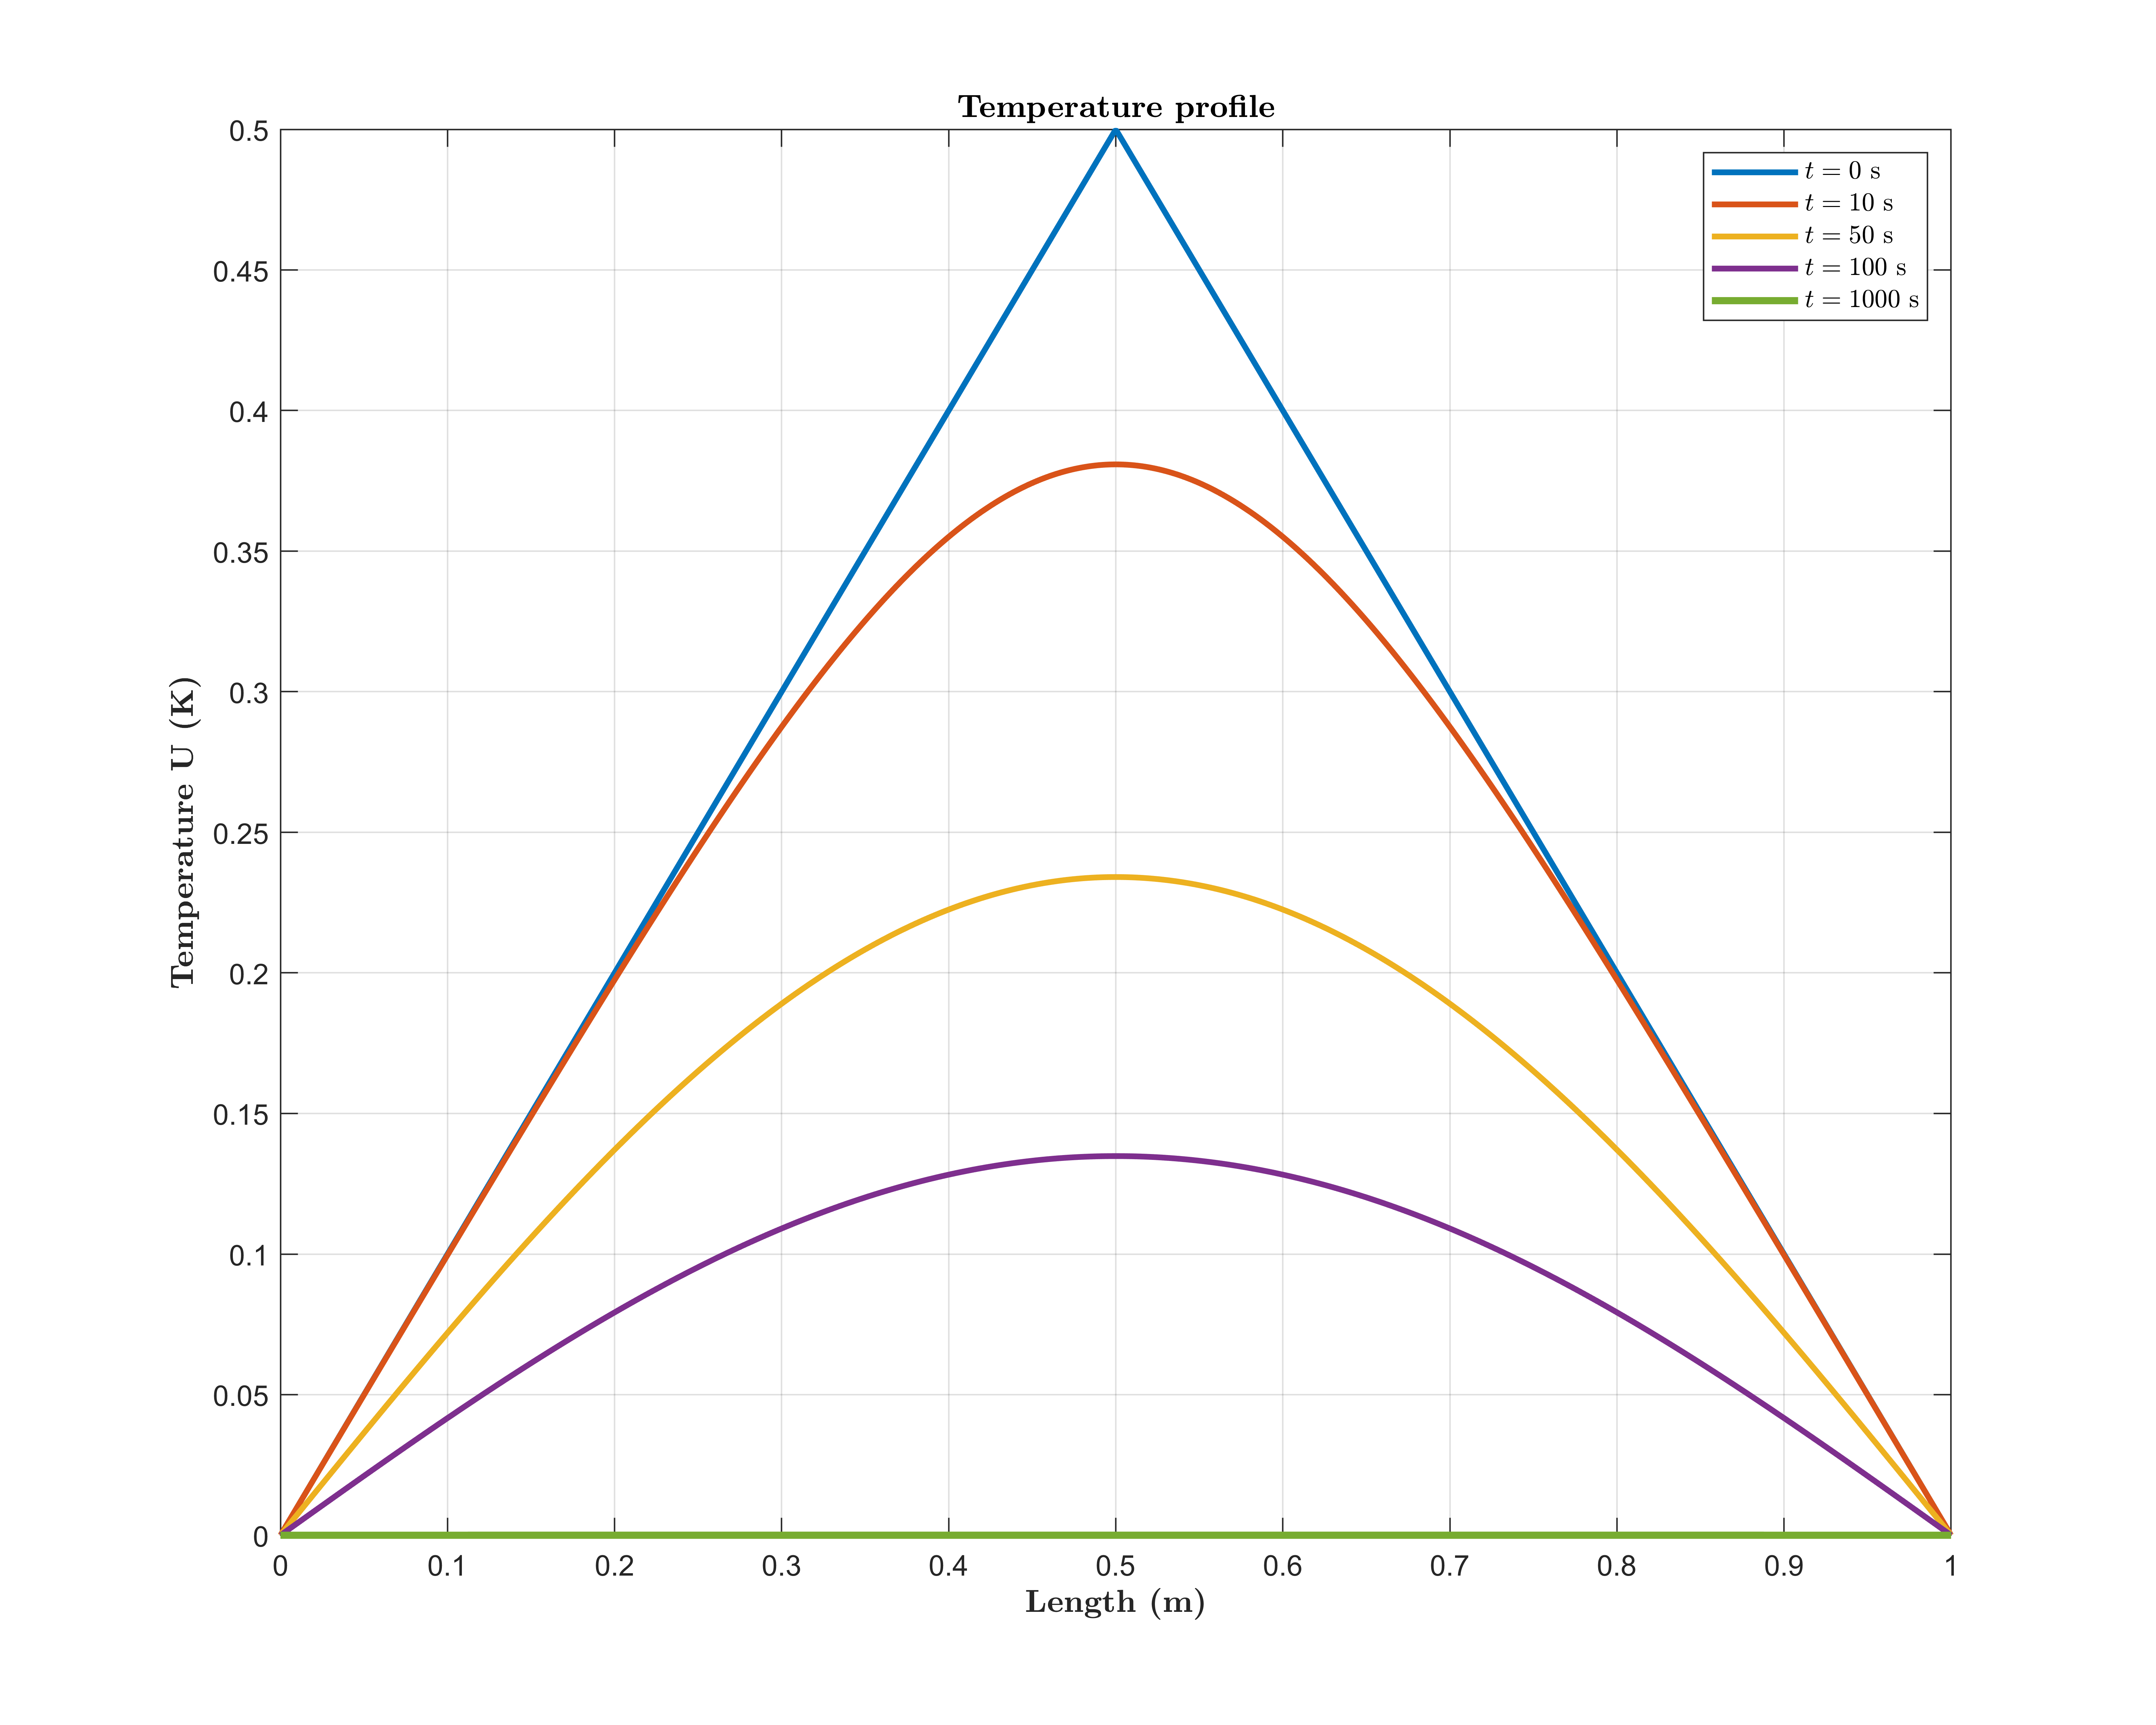
\includegraphics[width=0.8\textwidth]{Images/Problem_1_b.png}
\end{figure}\\
%1b ends
%%%%%%%%%%%%%%%%%%%%%%%%%%%%%%%%%%%%%%%%%%%%%%%%%%%%%%%%%%%%
%1c starts
\textbf{(c)}\quad
\begin{align*}
u(x,0) &= (u_L' - u_o') \cdot \left(\frac{x}{L}\right) + u'_0, \quad 0 < x < L \\
u(0,t) &= u_0 \\
u(L,t) &= u_L \\
\end{align*}
\emph{\textbf{Solution:}}\\
The solution is splitted into two parts, Steady state part and a time dependent part
\[
u(x,t) = u_s(x) + \theta(x,t)
\]
\[
\theta(x,t) = u(x,t) - u_s(x)
\]
Steady state governing equation:
\[
\frac{d^2u_s}{dx^2} = 0
\]
Boundary conditions,
\[
u_s(0) = u_o \quad u_s(L) = u_L
\]
\[
u_s(x) = \frac{u_L - u_o}{L}x + u_o
\]
\[
\theta(x,0) = g(x) = f(x) - u_s(x)
\]
\[
g(x) = \frac{u_L' - u_o'}{L}x + u_o'
\]
\[
\boxed{
\theta(x,t) = \sum_{n=1}^{\infty} B_n \cdot e^{-\alpha \cdot \left(\frac{n\pi}{2}\right)^2 \cdot t} \cdot \sin\left(\frac{n\pi x}{L}\right)
}
\]
\[
\boxed{
B_n = \frac{2}{L} \int_{0}^{L} g(x) \cdot \sin\left(\frac{n\pi}{L}x\right) \, dx
}
\]
solving for \(B_n\), it is split into \(B_1\), \(B_2\), \(B_3\), and \(B_4\) for convenience,
\[
B_1 = \frac{{(u_o' - u_L')}}{{n\pi}} \cdot L \cdot \cos(n\pi)
\]
\[
B_2 = \frac{{L \cdot u_o'}}{{n\pi}} \cdot (1 - \cos(n\pi))
\]
\[
B_3 = \frac{{(u_o - u_L)}}{{n\pi}} \cdot L \cdot \cos(n\pi)
\]
\[
B_4 = \frac{{L \cdot u_o}}{{n\pi}} \cdot (1 - \cos(n\pi))
\]
\[
B_n = \frac{2}{L} \cdot (B_1 + B_2 - B_3 - B_4)
\]
\[
\boxed{
B_n = \frac{2}{L} \cdot (\frac{{(u_o' - u_L')}}{{n\pi}} \cdot L \cdot \cos(n\pi) + \frac{{L \cdot u_o'}}{{n\pi}} \cdot (1 - \cos(n\pi)) - \frac{{(u_o - u_L)}}{{n\pi}} \cdot L \cdot \cos(n\pi) - \frac{{L \cdot u_o}}{{n\pi}} \cdot (1 - \cos(n\pi)))
}
\]
The total solution,
\[
u(x,t) = \frac{u_L - u_o}{L}x + u_o + \sum_{n=1}^{\infty} B_n \cdot e^{-\alpha \cdot \left(\frac{n\pi}{2}\right)^2 \cdot t} \cdot \sin\left(\frac{n\pi x}{L}\right)
\]
\[
\boxed{
\begin{aligned}
u(x,t) = & \frac{u_L - u_o}{L}x + u_o \\
& + \sum_{n=1}^{\infty} \frac{2}{L} \cdot \Bigg( \frac{(u_o' - u_L')}{n\pi} \cdot L \cdot \cos(n\pi) \\
& + \frac{L \cdot u_o'}{n\pi} \cdot (1 - \cos(n\pi)) - \frac{(u_o - u_L)}{n\pi} \cdot L \cdot \cos(n\pi) \\
& - \frac{L \cdot u_o}{n\pi} \cdot (1 - \cos(n\pi)) \Bigg) \cdot e^{-\alpha \cdot \left(\frac{n\pi}{2}\right)^2 \cdot t} \cdot \sin\left(\frac{n\pi x}{L}\right)
\end{aligned}
}
\]
The values are assumed for plotting, \\
$u_o = 50\, \text{K}$ \\
$u_L = 100\, \text{K}$ \\
$u_o' = 100\, \text{K}$ \\
$u_L' = 200\, \text{K}$ \\
Thermal diffusivity, $\alpha = 1.115 \times 10^{-3}\, \text{m}^2/\text{s}$ \\
Length of the domain, $L = 1\, \text{m}$ \\
The plot is shown below:\\
\begin{figure}[htbp]
    \centering
    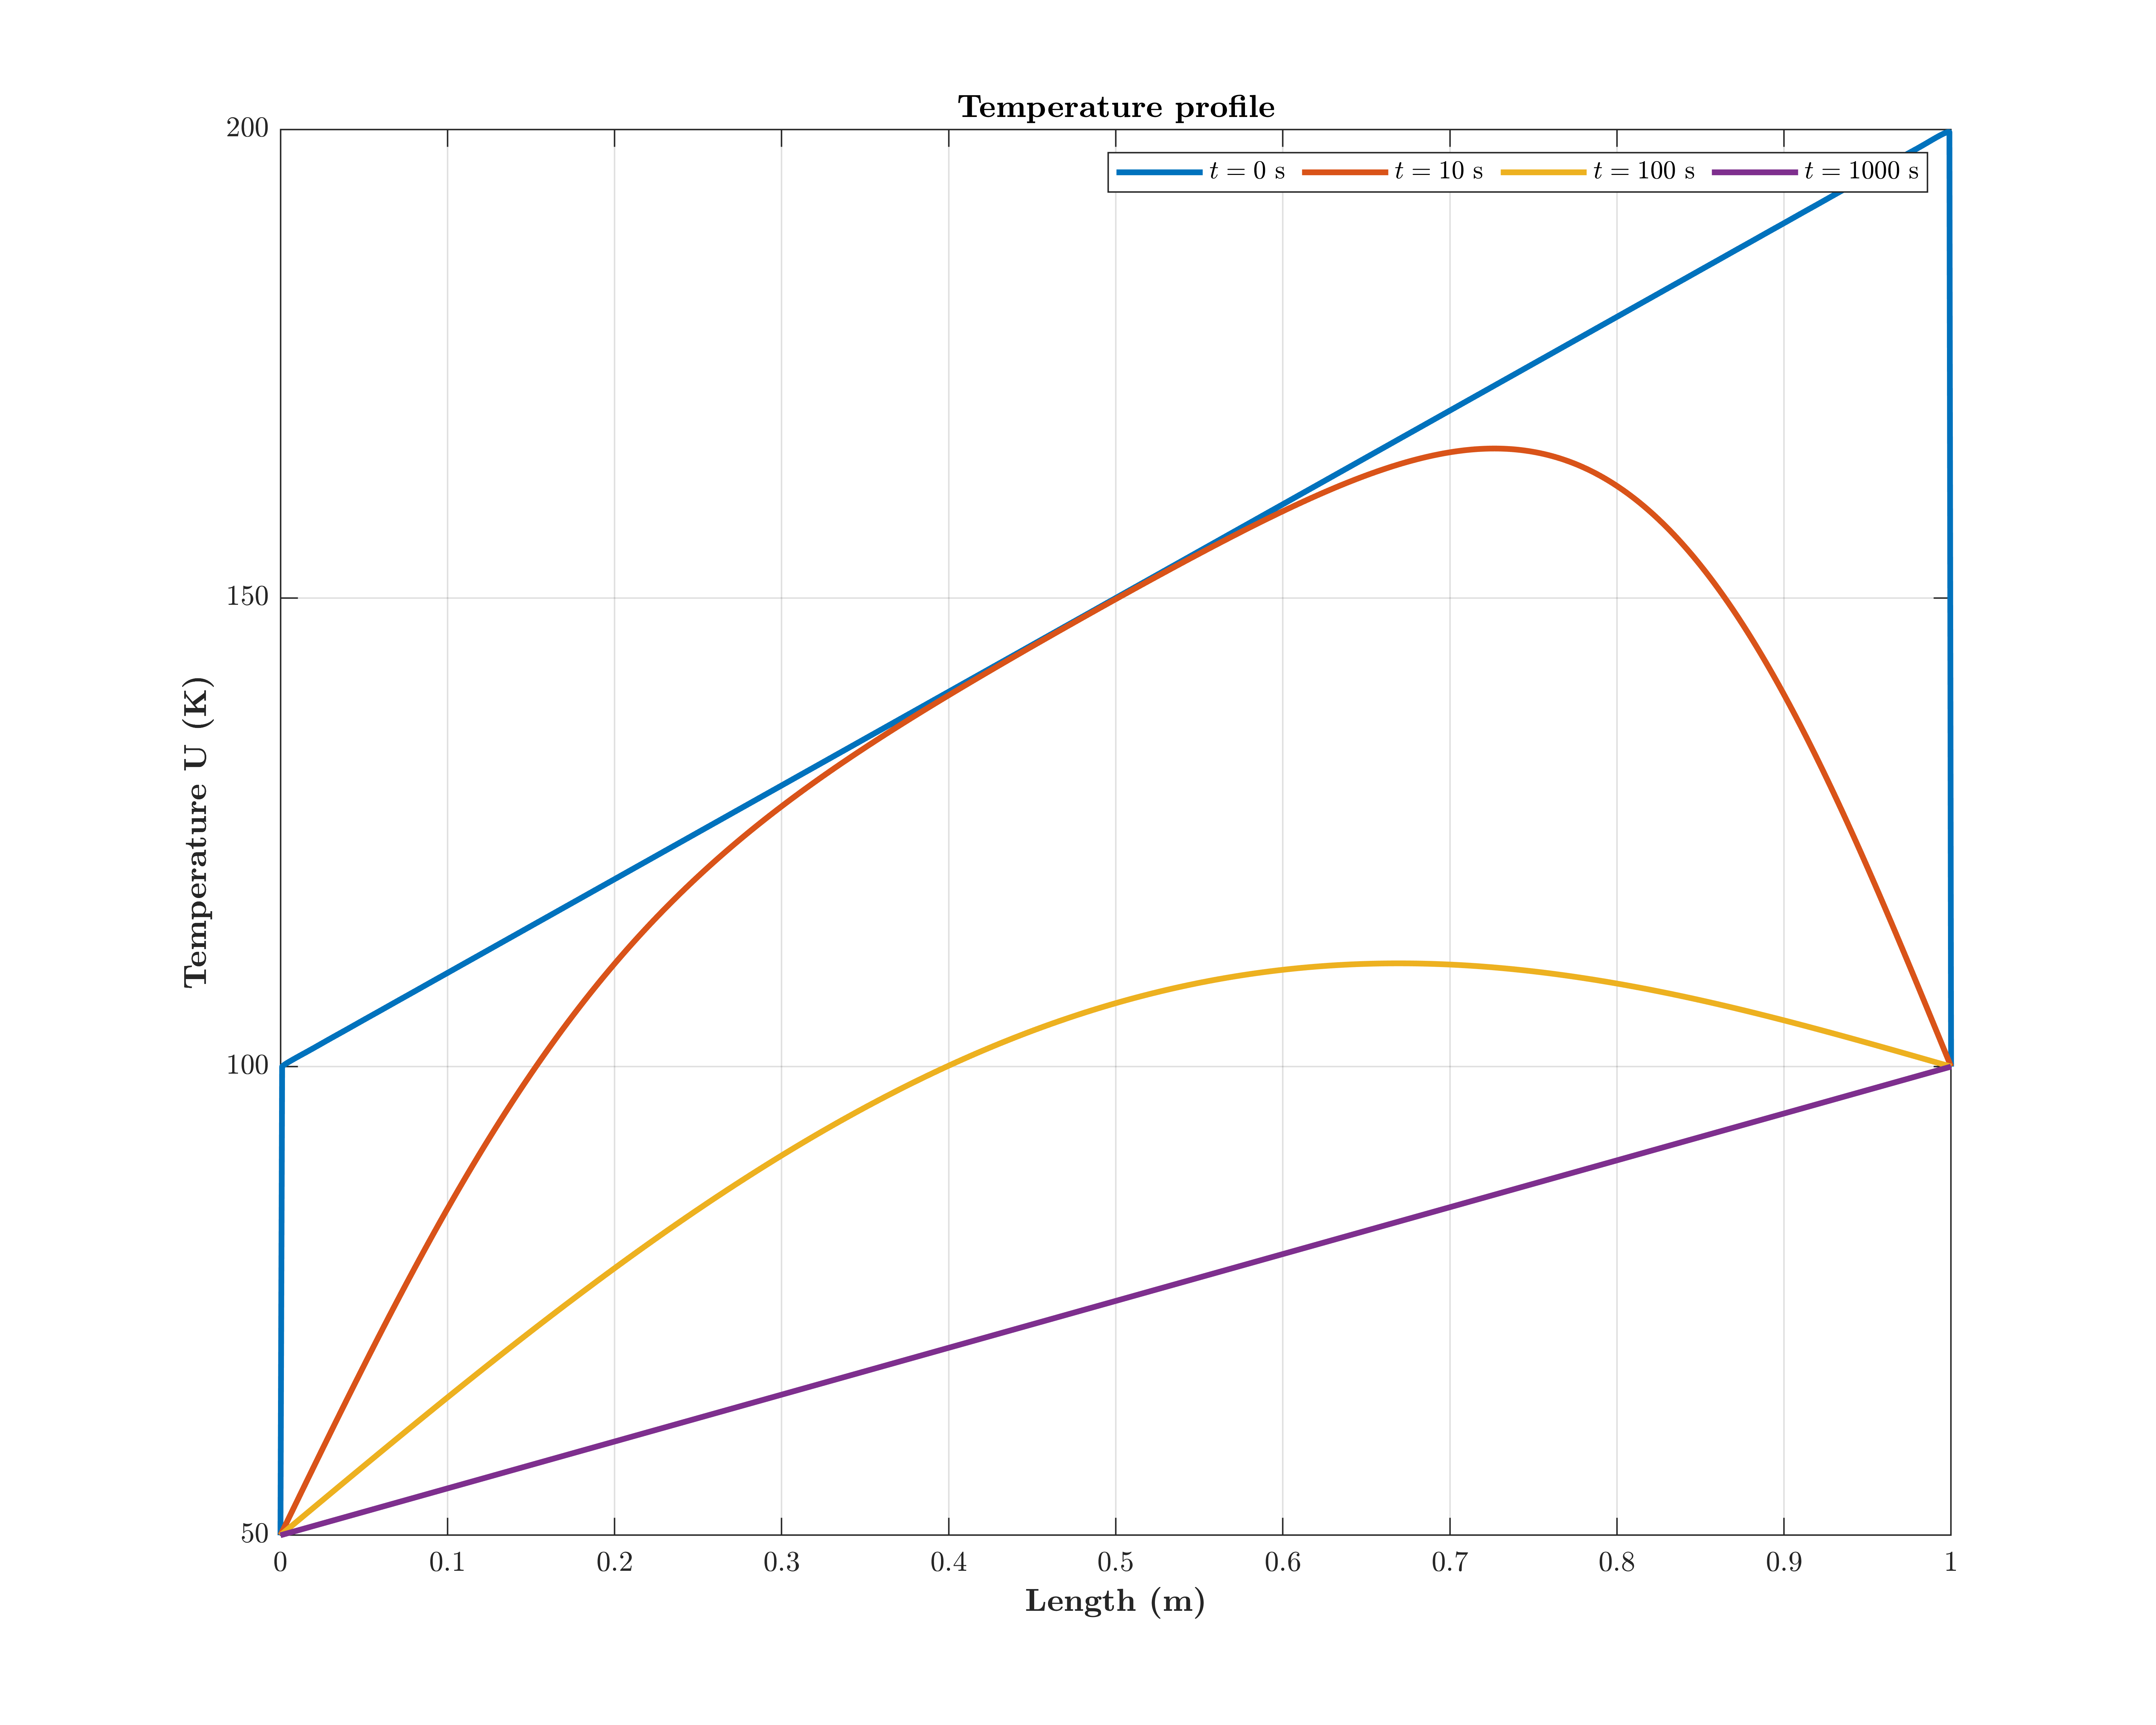
\includegraphics[width=0.8\textwidth]{Images/Problem_1_c.png}
\end{figure}\\
%1c ends
%%%%%%%%%%%%%%%%%%%%%%%%%%%%%%%%%%%%%%%%%%%%%%%%%
\pagebreak
%1d starts
\\
\textbf{(d)}\quad
\begin{align*}
u(x,0) &= \begin{cases}
u_l, & 0 < x \leq \frac{L}{2} \\
u_r, & \frac{L}{2} < x < L \\
\end{cases}\\
u(0,t) &= u_l \\
u(L,t) &= u_r \\
\end{align*}
\emph{\textbf{Solution:}}\\
Following a similar procedure, we can find the steady state solution,
\[
u_s(x) = \frac{u_r - u_L}{L}x + u_L
\]
\[
g(x) = \frac{u_r - u_L}{L}x \quad 0<x\le \frac{L}{2}
\]
\[
g(x) = u_r - \frac{u_r - u_L}{L}x - u_L \quad \frac{L}{2}<x\le L
\]
\[
B_n = \frac{2}{L}\int_{0}^{L} g(x)\sin\left(\frac{n\pi}{L}\right) \,dx
\]
\[
\boxed{
B_n = \frac{{2(u_r - u_L)}}{{n\pi}} \cdot \cos\left(\frac{{n\pi}}{{2}}\right)
}
\]
\[
\boxed{
\theta(x,t) = \sum_{n=1}^{\infty} B_n \cdot e^{-\alpha \cdot \left(\frac{n\pi}{2}\right)^2 \cdot t} \cdot \sin\left(\frac{n\pi x}{L}\right)
}
\]
The total solution,
\[
\boxed{
u(x,t) = \frac{u_r - u_L}{L}x + u_L + \sum_{n=1}^{\infty} \frac{{2(u_r - u_L)}}{{n\pi}} \cdot \cos\left(\frac{{n\pi}}{{2}}\right) \cdot e^{-\alpha \cdot \left(\frac{n\pi}{2}\right)^2 \cdot t} \cdot \sin\left(\frac{n\pi x}{L}\right)
}
\]
The values are assumed for plotting, \\
Thermal diffusivity, $\alpha = 1.115 \times 10^{-3}\, \text{m}^2/\text{s}$ \\
Length of the domain, $L = 1\, \text{m}$ \\
$u_r = 100\, \text{K}$ \\
$u_L = -100\, \text{K}$ \\
The plot is shown below:\\
\begin{figure}[htbp]
    \centering
    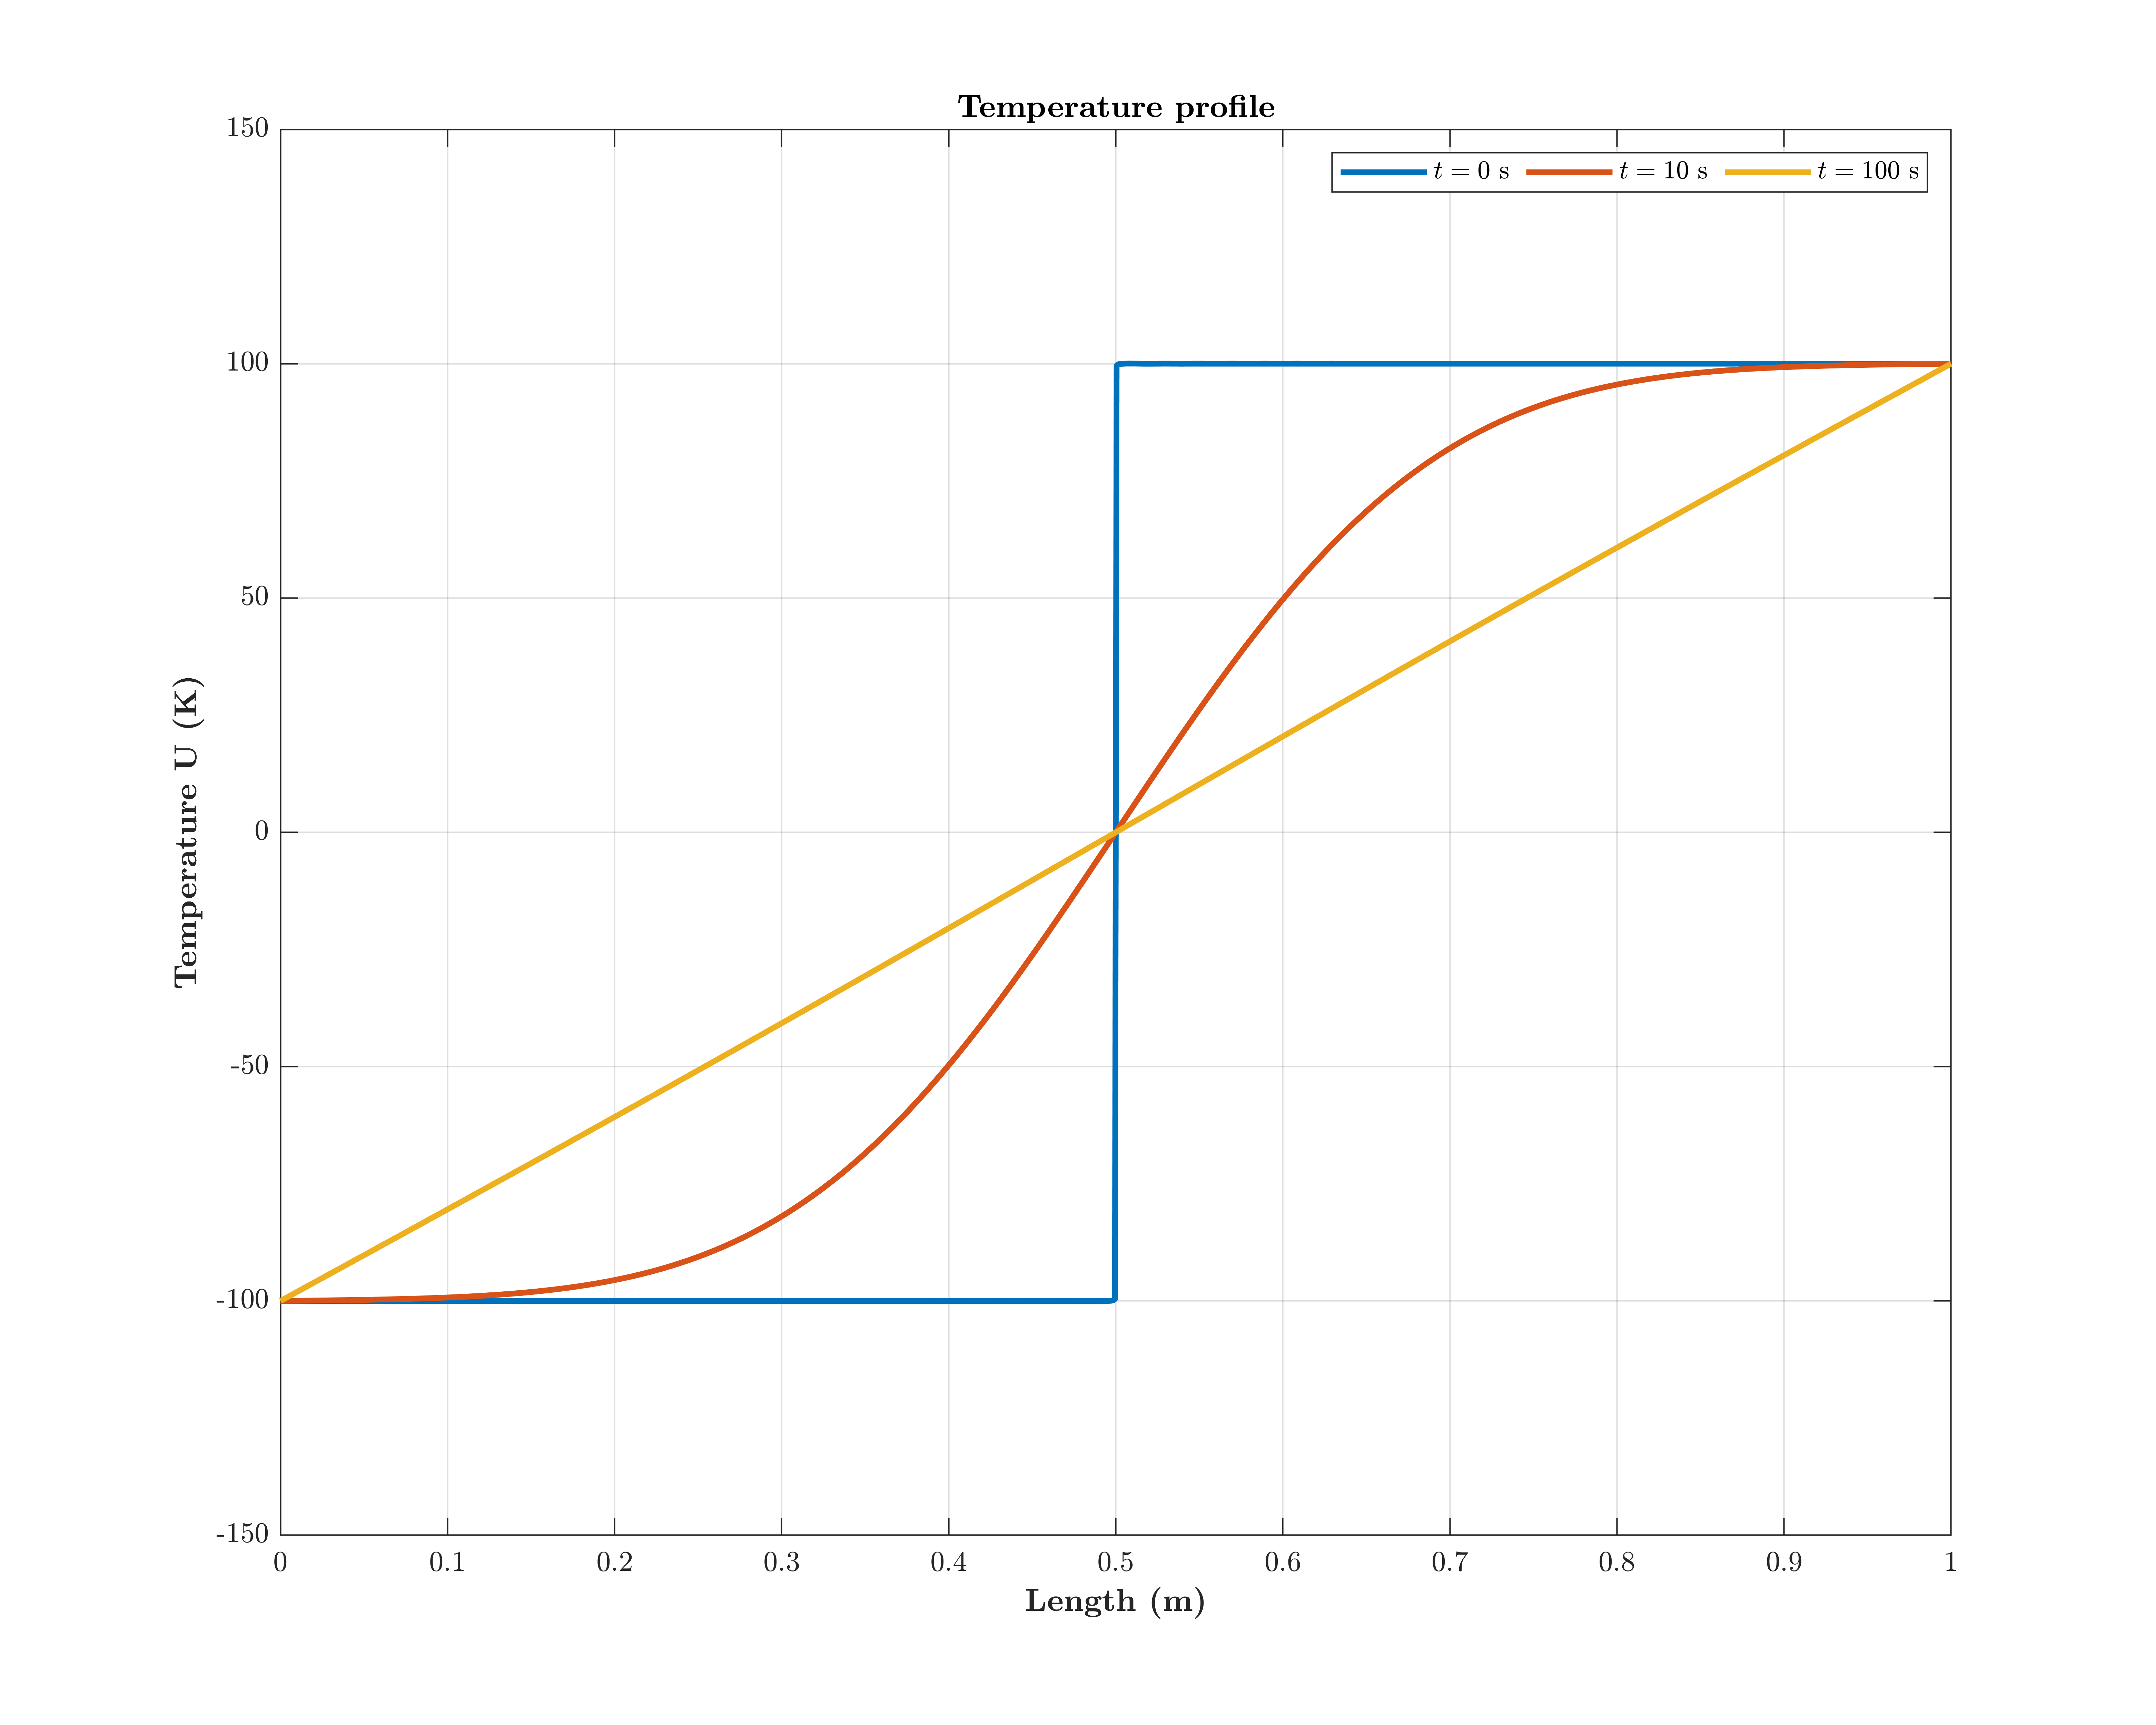
\includegraphics[width=0.8\textwidth]{Images/Problem_1_d.png}
\end{figure}\\
%1d ends
%%%%%%%%%%%%%%%%%%%%%%%%%%%%%%%%%%%%%%%%%%%%%%%%%%%%%%%%%%%%%%%%%%%%%%%%%%%%%%%%%%%%%%%%%%%%%%%

%1e starts
\textbf{(e)}\quad
\begin{align*}
u(x,0) &= U, \quad 0 < x < L \\
u(0,t) &= u_0 \\
\left. \frac{\partial u}{\partial x} \right|_{x=L} &= 0
\end{align*}
\emph{\textbf{Solution:}}\\
Applying a transformation to make the boundary conditions homogeneous,
\[
\theta(x,t) = u(x,t) - u_o
\]
Governing equation
\[
\frac{\partial\theta}{\partial t} = \alpha \frac{\partial^2\theta}{\partial x^2}
\]
Initial condition
\[
\theta(x,0) = U - u_o
\]
Boundary conditions
\[
\theta(0,t) = 0
\]
\[
\frac{\partial \theta}{\partial x}\Big|_{x=L} = 0
\]
Applying the method of separation of variables,
\[
\theta(x,t) = X(x) \cdot T(t)
\]
Substituting this into the governing equation and solving,
\[
\boxed{
\theta_n = \sum_{n=1}^{\infty} B_n \cdot e^{-\alpha \cdot \left(\frac{n\pi}{2}\right)^2 \cdot t} \cdot \sin(\lambda_n x)
}
\]
where $\lambda_n$ is
\[
\boxed{
\lambda_n = \frac{(2n-1)\pi}{2L}
}
\]
\[
\boxed{
B_n = \frac{2(U-u_o)}{L\lambda_n}(1 - \cos(\lambda_n L))
}
\]
The final solution,
\[
\boxed{
u(x,t) = u_o + \sum_{n=1}^{\infty} \frac{2(U-u_o)}{L\lambda_n}(1 - \cos(\lambda_n L)) \cdot e^{-\alpha \cdot \left(\frac{n\pi}{2}\right)^2 \cdot t} \cdot \sin(\lambda_n x)
}
\]
The values are assumed for plotting, \\
Thermal diffusivity, $\alpha = 1.115 \times 10^{-3}\, \text{m}^2/\text{s}$ \\
Length of the domain, $L = 1\, \text{m}$ \\
Initial temperature, $U = 50\, \text{K}$ \\
Temperature at $x = 0$. $u_o = 10\, \text{K}$ \\
The plot is shown below:\\
\begin{figure}[htbp]
    \centering
    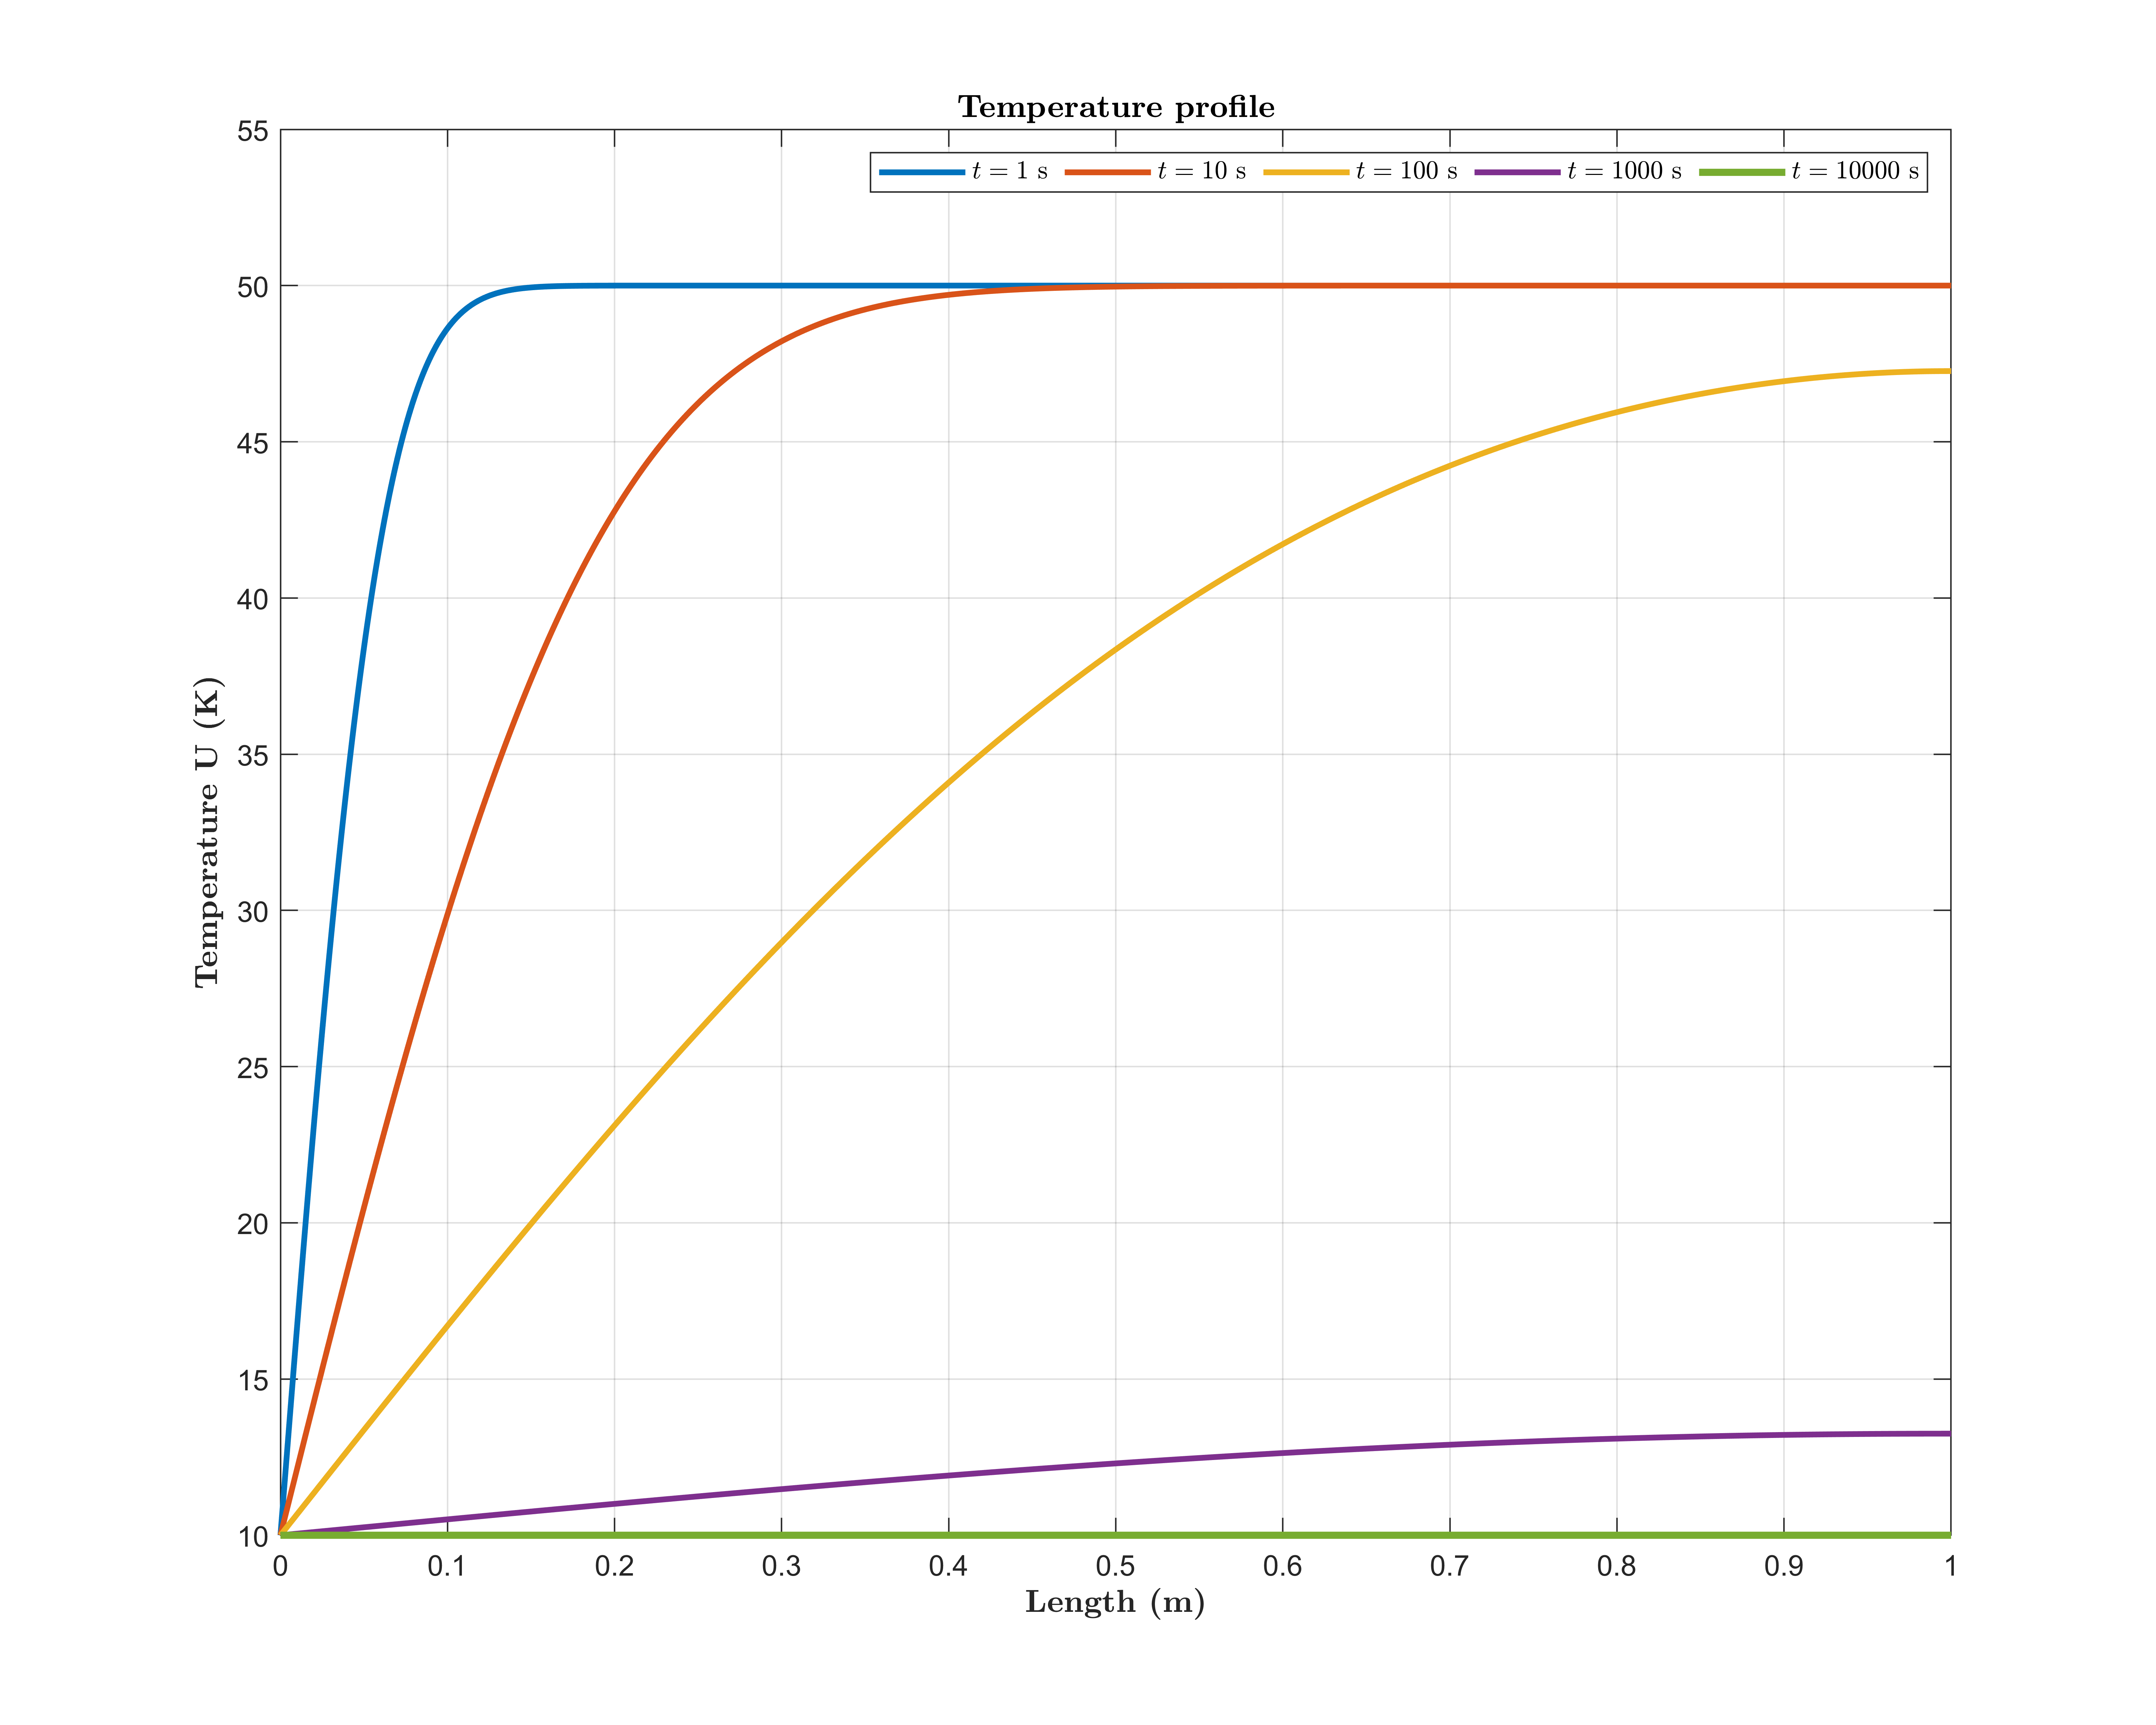
\includegraphics[width=0.8\textwidth]{Images/Problem_1_e.png}
\end{figure}\\
%1e ends
%%%%%%%%%%%%%%%%%%%%%%%%%%%%%%%%%%%%%%%%%%%%%%%%%%%%%%%%%%%%%%%%%%%%%%%%%%%%%%%%%%%%%%%%%%%%%%%%
\\
\newpage
%1f starts
\textbf{(f)}\quad
\begin{align*}
u(x,0) &= \frac{U}{2} \left(1 + \cos \frac{\pi x}{L}\right), \quad 0 < x < L \\
\left. \frac{\partial u}{\partial x} \right|_{x=0} &= 0 \\
\left. \frac{\partial u}{\partial x} \right|_{x=L} &= 0
\end{align*}
\emph{\textbf{Solution:}}\\
Following a similar procedure except for the boundary conditions from the previous problem $e$,
we can get the final solution as,
\[
u(x,t) = \sum_{n=0}^{\infty} a_n \cdot e^{-\alpha \cdot \left(\frac{n\pi}{L}\right)^2 \cdot t} \cdot \cos\left(\frac{n\pi x}{L}\right)
\]

Only \(a_1\) and \(a_0\) exist,
\[
a_1 = \frac{2}{L} \int_{0}^{L} f(x) \cdot \cos\left(\frac{\pi x}{L}\right) \,dx
\]
\[
a_0 = \frac{2}{L} \int_{0}^{L} f(x) \,dx
\]

where \(f(x)\) is
\[
f(x) = \frac{U}{2} \left(1 + \cos\left(\frac{\pi x}{L}\right)\right)
\]

Solving for \(a_1\) and \(a_0\) and substituting in the final solution,
\[
\boxed{
u(x,t) = \frac{U}{2} \left(1 + e^{-\alpha \cdot \left(\frac{\pi}{L}\right)^2 \cdot t} \cdot \cos\left(\frac{\pi x}{L}\right)\right)
}
\]
The values are assumed for plotting, \\
Thermal diffusivity, $\alpha = 1.115 \times 10^{-3}\, \text{m}^2/\text{s}$ \\
Length of the domain, $L = 1\, \text{m}$ \\
$U = 50\, \text{K}$ \\
The plot is shown below:\\
\begin{figure}[htbp]
    \centering
    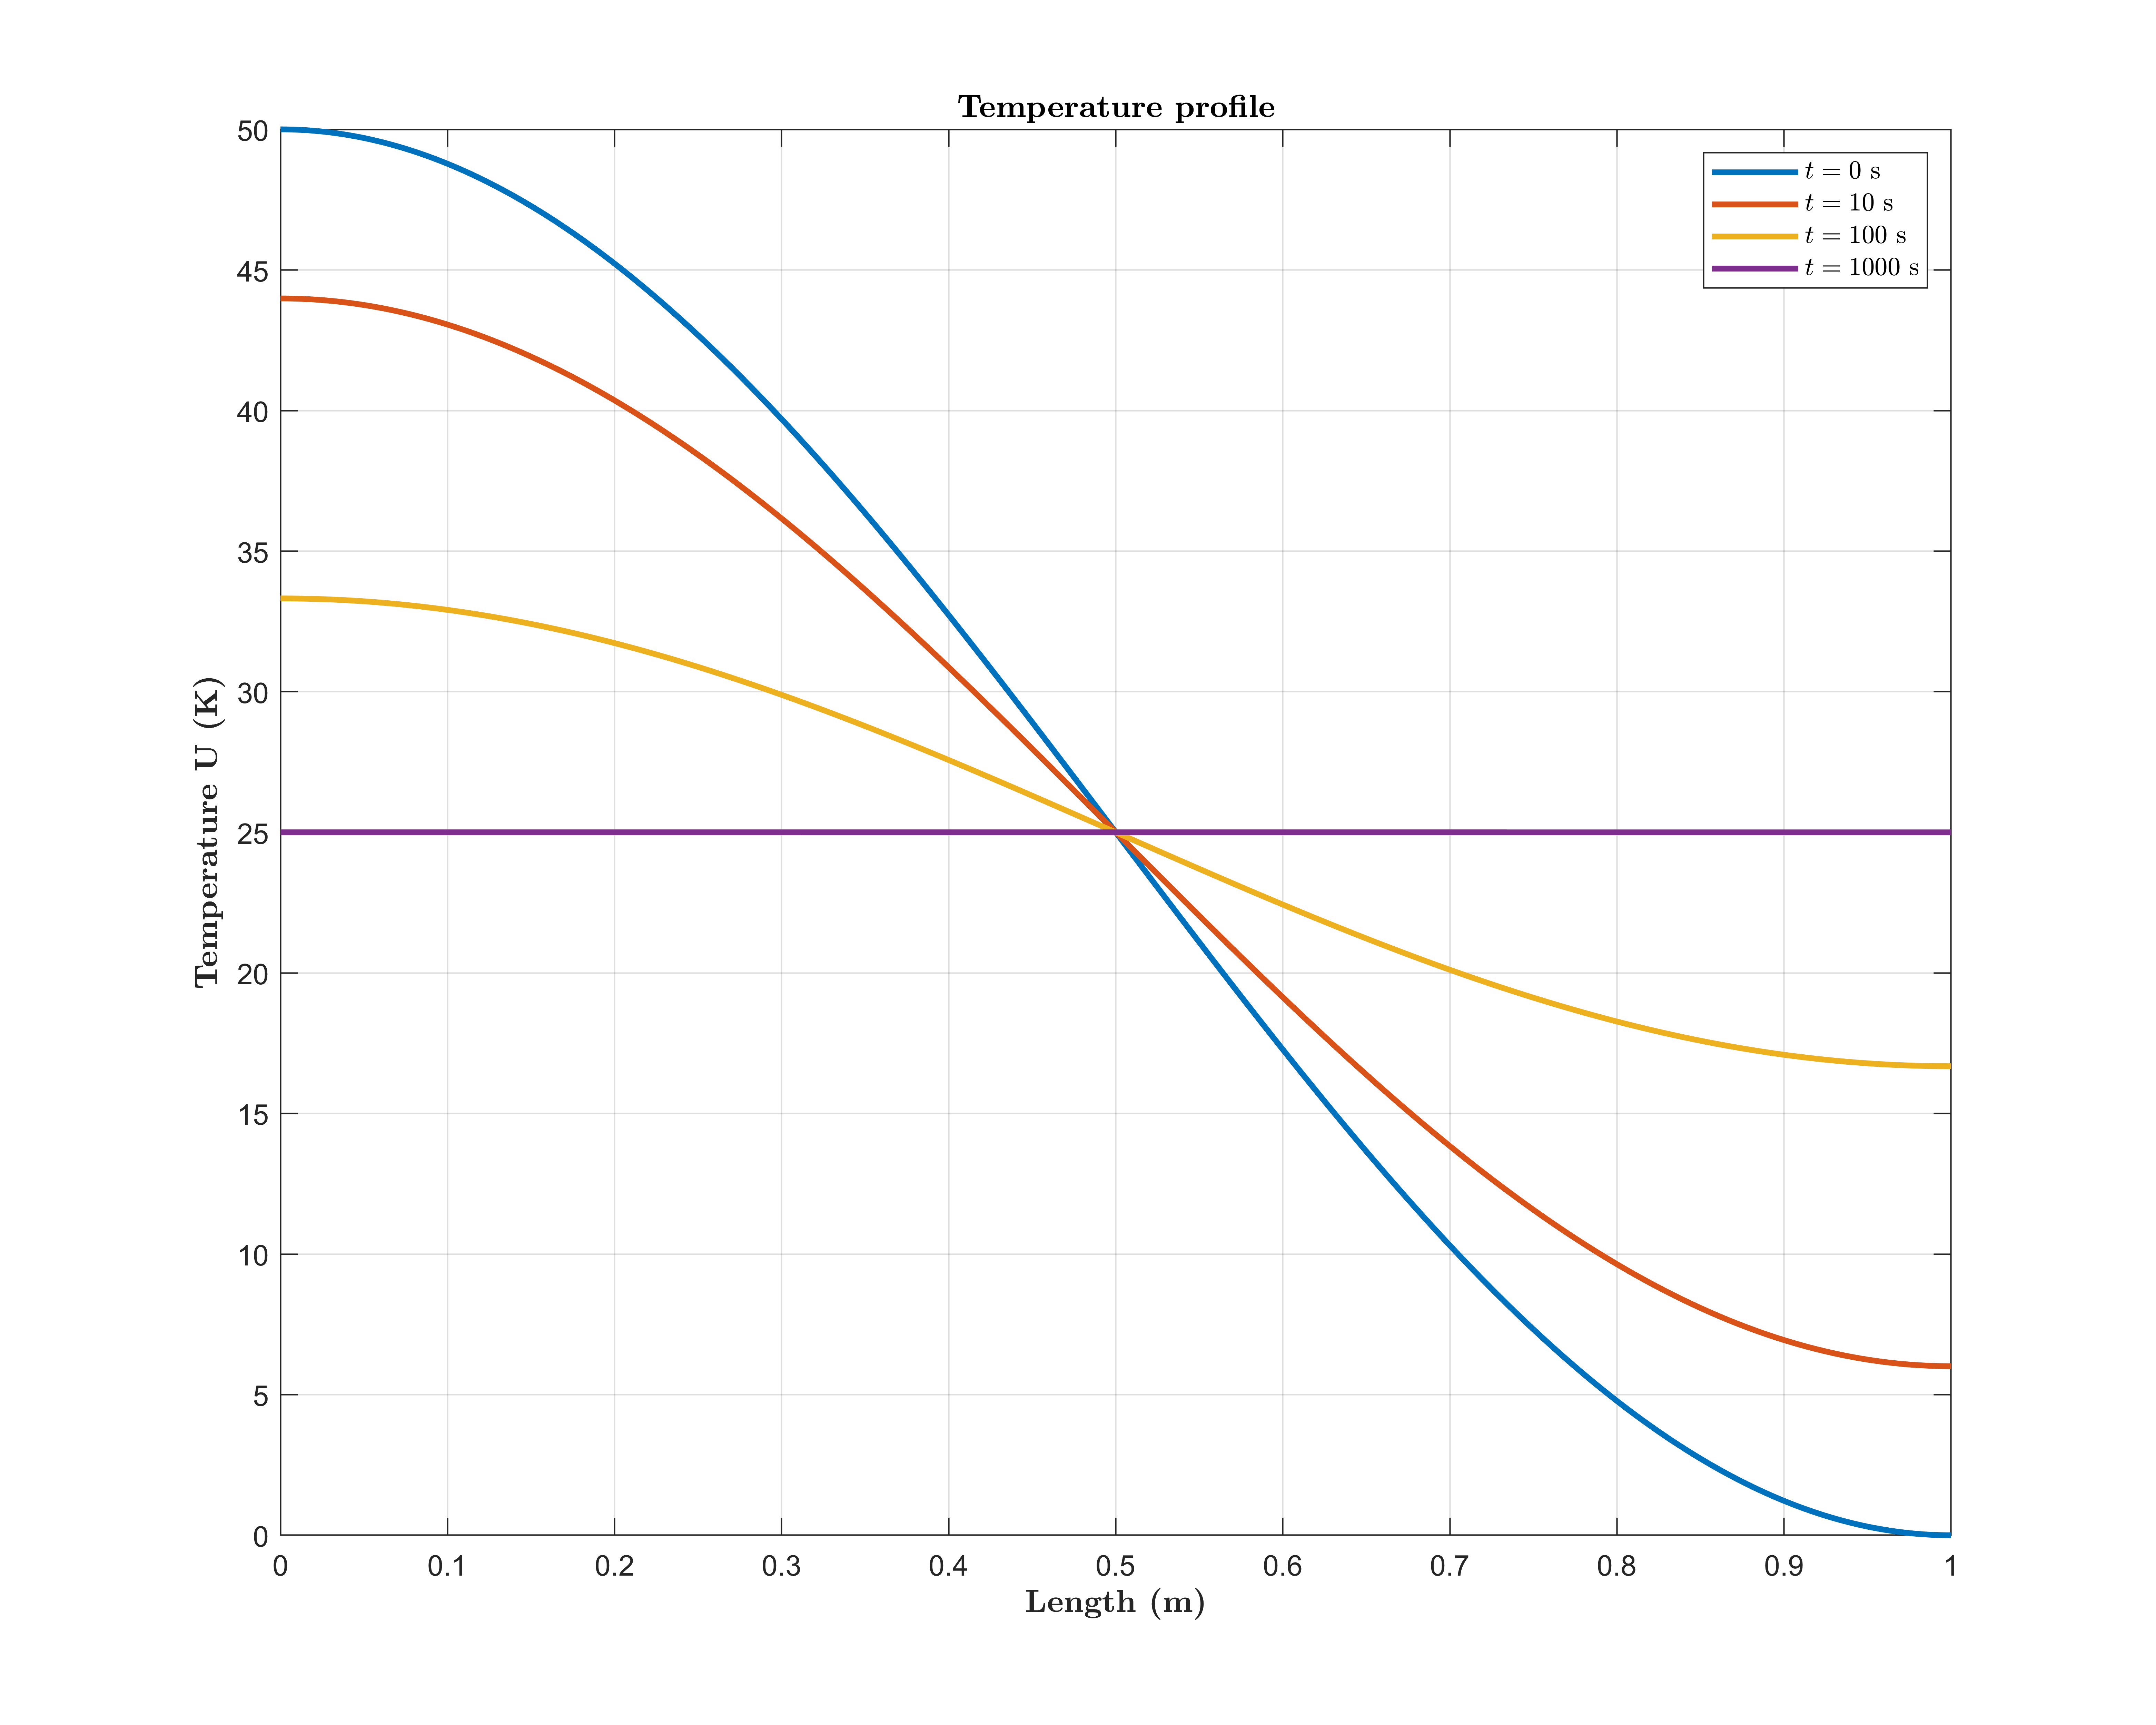
\includegraphics[width=0.8\textwidth]{Images/Problem_1_f.png}
\end{figure}\\
%1f ends
%%%%%%%%%%%%%%%%%%%%%%%%%%%%%%%%%%%%%%%%%%%%%%%%%%%%%%%%%%%%%%%%%%%%%%%%%%%%%%%%%%%%%%%%%%%%%%%%
%\pagebreak
%2nd problem starts
\item 
Solve the one-dimensional heat equation
\[
\frac{\partial u}{\partial t} = \alpha \frac{\partial^2 u}{\partial x^2} + \frac{\dot{q}_g}{c}, \quad 0 < x < L, \, t > 0
\]
in a finite domain for the following initial and boundary conditions:
\[
u(x,0) = f(x), \quad 0 < x < L
\]
\[
u(0,t) = u_0
\]
\[
u(L,t) = u_L
\]
\emph{\textbf{Solution:}}\\
The problem can be split into two parts,
\[
U(x, t) = \theta(x, t) + u_s(x)
\]
\[
\frac{\partial^2 \theta}{\partial x^2} + \frac{d^2 u_s}{dx^2} + \frac{\dot{q_g}}{\alpha c} = \frac{1}{\alpha}\frac{\partial\theta}{\partial t}
\]
\[
\frac{\partial^{2}\theta}{\partial x^{2}} = \frac{1}{\alpha} \frac{\partial\theta}{\partial t}
\]
\[
\frac{d^{2} u_s}{dx^{2}} + \frac{\dot{q_g}}{\alpha c} = 0
\]
Boundary conditions
\[
u_s(0) = u_o
\]
\[
u_s(L) = u_L
\]
\[
\theta(x,0) = f(x) - u_s(x)
\]
\[
\theta(0,t) = f(0) - u_o = 0
\]
\[
\theta(0,t) = f(L) - u_L = 0
\]

Solving for \(u_s\),
\[
u_s(x) = u_o + (u_L - u_o)\frac{x}{L} + \frac{\dot{q_g}x}{2 \alpha L}(L - x)
\]
For the time-dependent solution \(\theta(x,t)\), this can be solved using the method of separation of variables,
\[
\theta(x,t) = X(x) \cdot T(t)
\]
\[
X(x) = A_n \sin(\lambda_n x) + B_n \cos(\lambda_n x)
\]
\[
T(t) = C_n e^{-\alpha \lambda_n^2 t}
\]
\[
\theta(x,t) = \sum_{n=1}^{\infty} a_n e^{-\alpha \lambda_n^2 t} \sin(\lambda_n x)
\]
Substituting the boundary conditions and solving, we get,
\[
\lambda_n = \frac{n\pi}{L}
\]
\[
\boxed{
a_n = \frac{2}{L} \int_{0}^{L} (f(x) - u_s(x)) \sin(\lambda_n x)\,dx
}
\]
The total solution is,
\[
\boxed{
u(x,t) = \sum_{n=1}^{\infty} a_n e^{-\alpha \lambda_n^2 t} \sin(\lambda_n x) + u_o + (u_L - u_o)\frac{x}{L} + \frac{\dot{q_g}x}{2 \alpha L}(L - x)
}
\]
Let $f(x) = U$, calculating $a_n$
\begin{empheq}[box=\fbox]{align*}
\begin{split}
a_n = & \frac{U - u_0}{\lambda_n}(1 - \cos(\lambda_n)) \\
& - \left(\frac{\sin(\lambda_n L)}{\lambda_n^2} - \frac{L \cos(\lambda_n L)}{\lambda_n}\right)\left(\frac{u_L - u_0}{L} + \frac{\dot{q}_g L}{2 \alpha L}\right) \\
& - \left(\frac{\dot{q}_g}{2 \alpha L}\right)\left(\frac{L^2 \cos(\lambda_n L)}{\lambda_n} - \frac{2 L \sin(\lambda_n L)}{\lambda_n^2} - \frac{2 \cos(\lambda_n L)}{\lambda_n^3} + \frac{2}{\lambda_n^3}\right)
\end{split}
\end{empheq}
Substituting $a_n$ in the $u(x,t)$, we can get a solution for plotting, \\
The values are assumed for plotting, \\
Thermal diffusivity, $\alpha = 1.115 \times 10^{-3}\, \text{m}^2/\text{s}$ \\
Length of the domain, $L = 1\, \text{m}$ \\
$U = 100\, \text{K}$ \\
$u_o = 50\, \text{K}$ \\
$u_L = 50\, \text{K}$ \\
Heat generation, $\dot{q_g} = 1\, \text{W}/\text{m}^3$ \\
$c = 1$ \\
\newpage
The plot is shown below:\\
\begin{figure}[htbp]
    \centering
    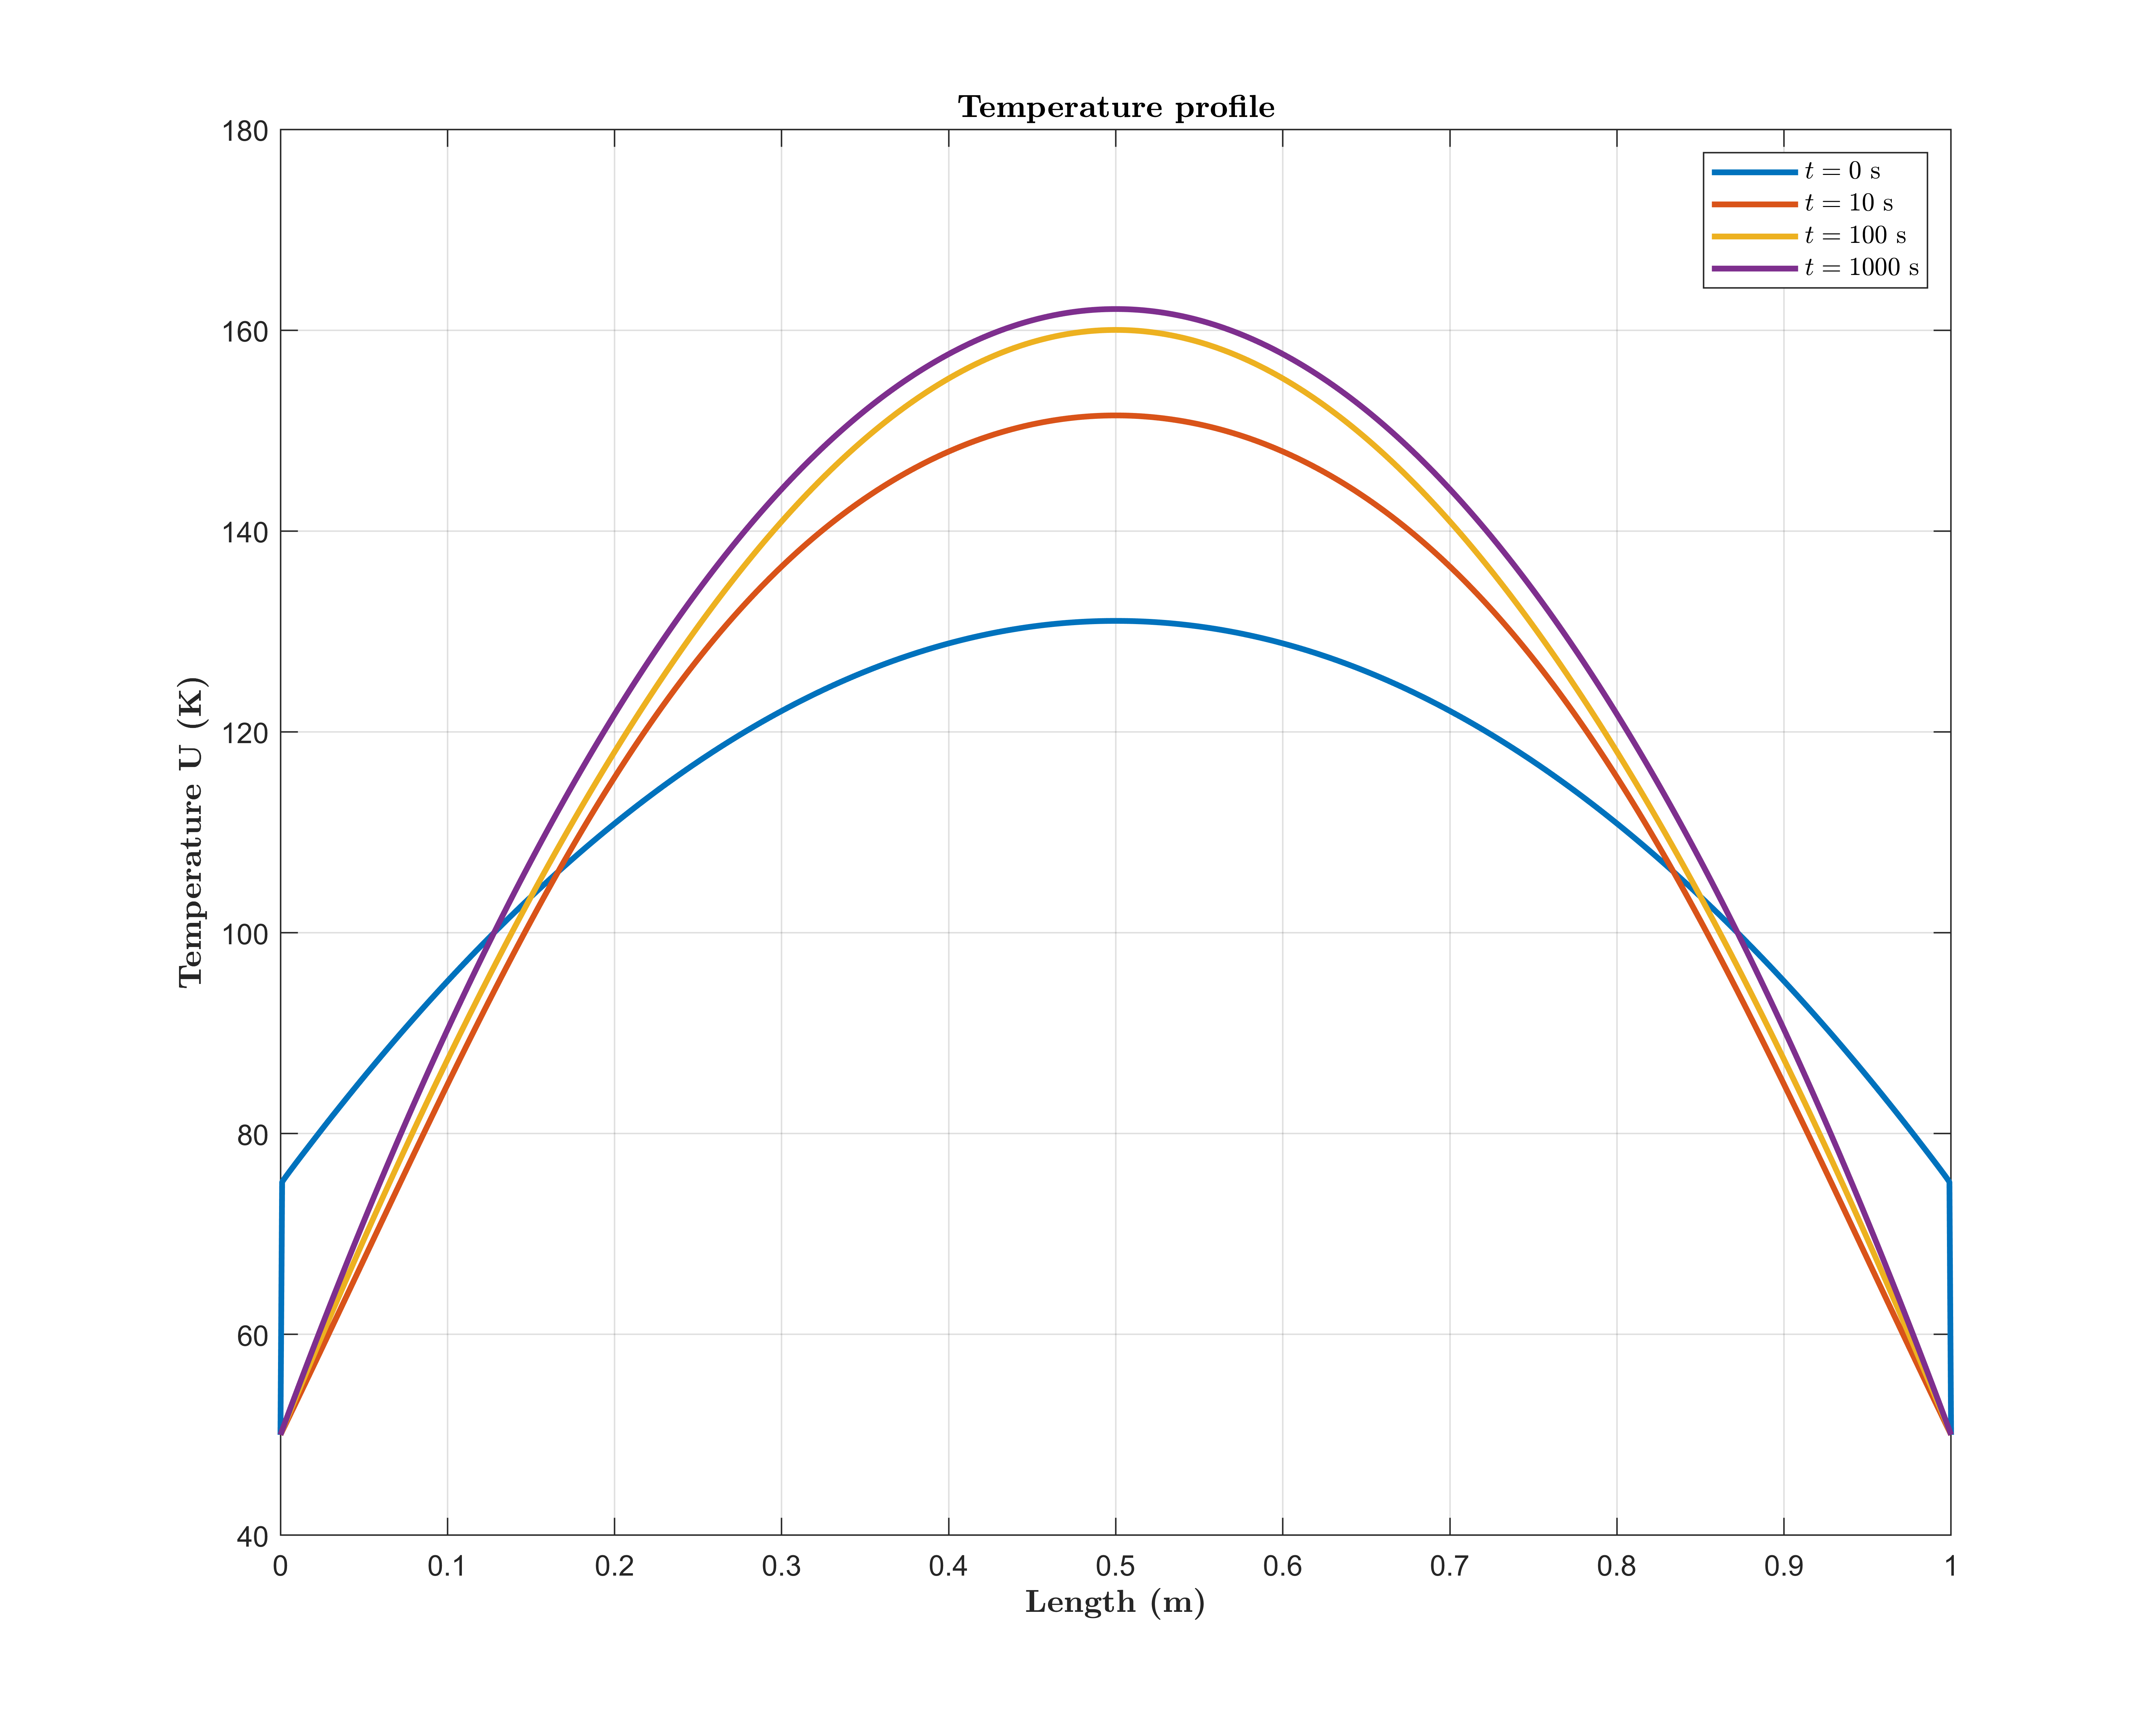
\includegraphics[width=0.8\textwidth]{Images/Problem_2.png}
\end{figure}\\
%2nd problem ends
%%%%%%%%%%%%%%%%%%%%%%%%%%%%%%%%%%%%%%%%%%%%%%%%%%%%%%%%%%%%%%%%%%%%%%%%%%%%%%%%%%%%%%%%%%%%%%%%
%3rd Problem starts
%3a Problem starts
\item 
Solve the one-dimensional heat equation
\[
\frac{\partial u}{\partial t} = \alpha \frac{\partial^2 u}{\partial x^2}, \quad -\infty < x < \infty, \, t > 0
\]
in an infinite domain for the following initial conditions:\\
\textbf{(a)}\quad
\begin{align*}
u(x,0) &= \begin{cases}
\cos x, & \text{if } x \leq |\pi| \\
0, & \text{if } x > |\pi|
\end{cases}
\end{align*}
\emph{\textbf{Solution:}}\\
From
\[
u(x,t) = \frac{1}{\sqrt{\pi}} \int_{-\infty}^{\infty} f(x - k\sqrt{4\alpha t}) e^{-k^2}\,dk
\]

For our problem,
\[
u(x,t) = \frac{1}{\sqrt{4\alpha t \pi}} \int_{-\pi}^{\pi} \cos(x - k\sqrt{4\alpha t}) e^{-k^2}\,dk
\]

Using $\cos(A+B) = \cos(A)\cos(B) - \sin(A)\sin(B)$ and simplifying,
\[
u(x,t) = \frac{1}{\sqrt{\pi}} \int_{-\pi}^{\pi} \cos(x)\cos(k\sqrt{4\alpha t)} e^{-k^2}\,dk
\]

Integrating the right-hand side,
\[
\boxed{
u(x,t) = \frac{\cos(x)e^{-\alpha t}}{2} \left[\text{erf}(\pi - i\sqrt{\alpha t}) - \text{erf}(-\pi - i\sqrt{\alpha t})\right]
}
\]

For plotting, considering only real values, the equation becomes,
\[
u(x,t) = \frac{\cos(x)e^{-\alpha t}}{2}
\]

The values assumed for plotting, \\
Thermal diffusivity, $\alpha = 1.115 \times 10^{-3}\, \text{m}^2/\text{s}$ \\
The plot is shown below:
\begin{figure}[htbp]
    \centering
    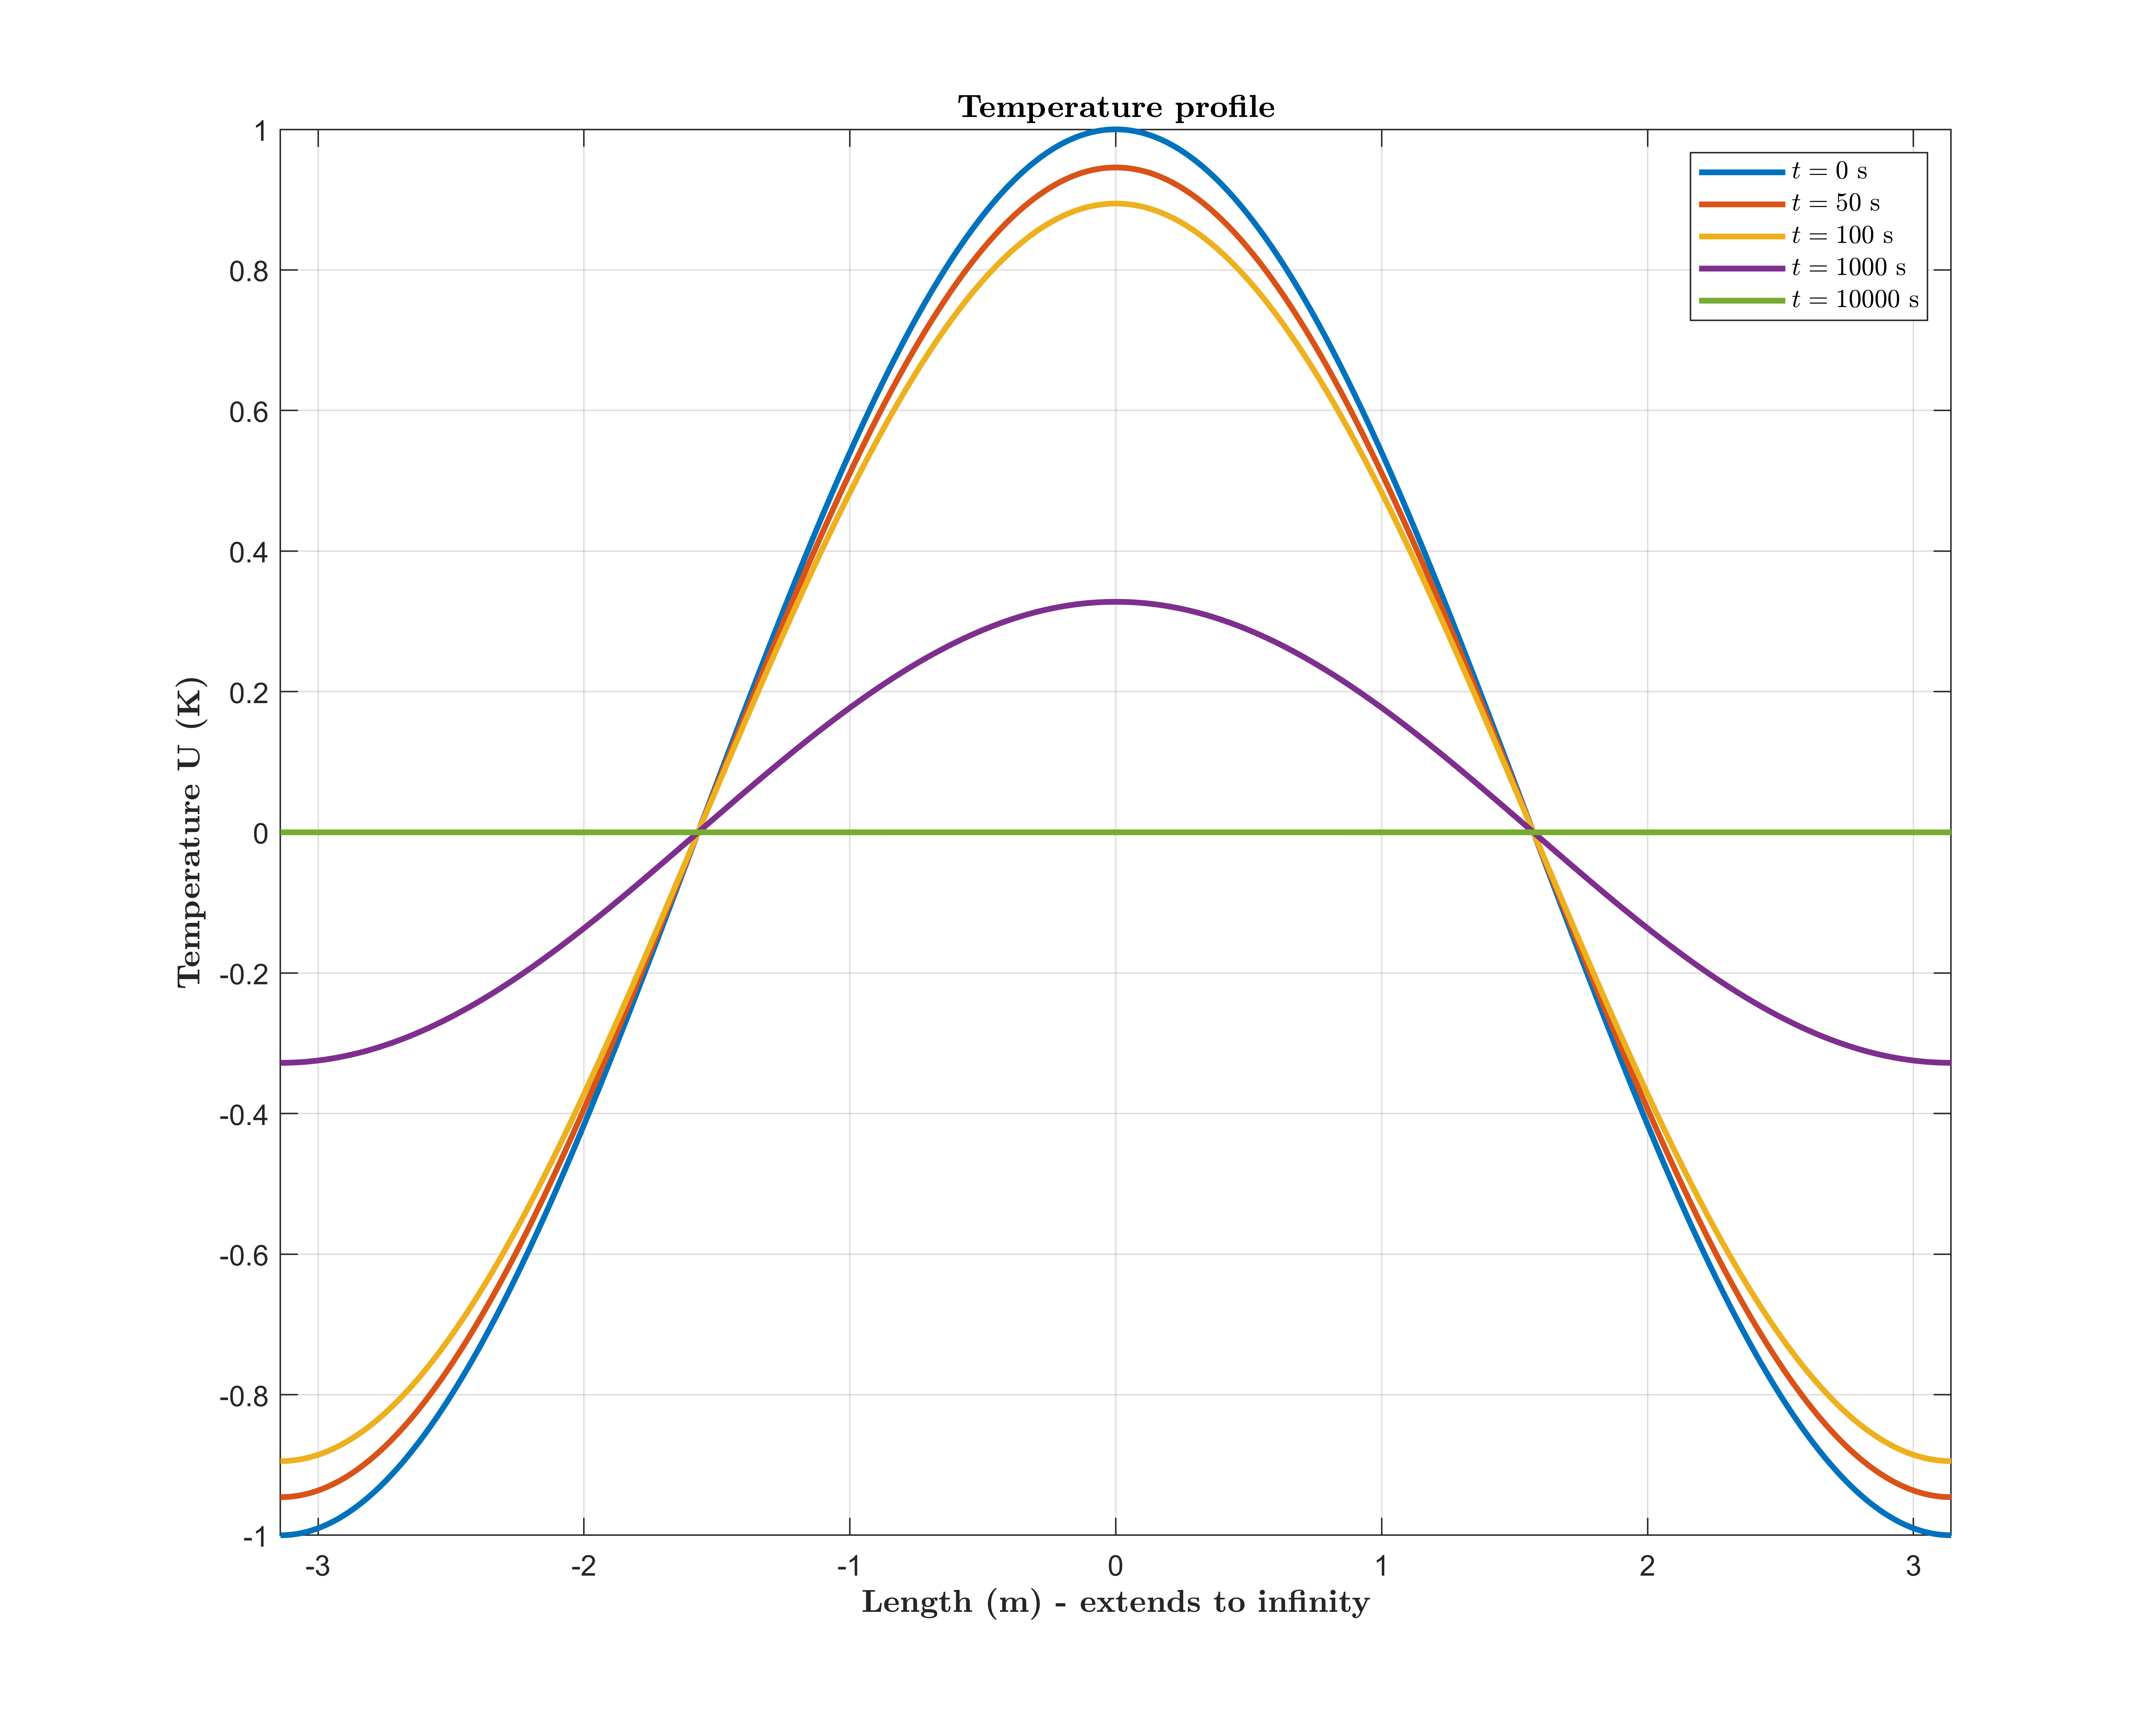
\includegraphics[width=0.8\textwidth]{Images/Problem_3_a.png}
\end{figure}

%3a Problem ends
%%%%%%%%%%%%%%%%%%%%%%%%%%%%%%%%%%%%%%%%%%%%%%%%%%%%%%%%%%%%%%%%%%%%%%%%%%%%%%%%%%%%%%%%%%%%%%%
%3b Problem starts
\textbf{(b)}\quad
\begin{align*}
u(x,0) &= \begin{cases}
u_l, & \text{if } x \leq 0 \\
u_r, & \text{if } x > 0
\end{cases}
\end{align*}
\emph{\textbf{Solution:}}\\
From
\[
u(x,t) = \frac{1}{\sqrt{4\alpha t \pi}} \int_{-\infty}^{\infty} f(s) e^{\frac{-(s-x)^2}{4\alpha t}}\,ds
\]

For our problem,
\[
u(x,t) = \frac{1}{\sqrt{4\alpha t \pi}} \int_{-\infty}^{0} u_l e^{\frac{-(s-x)^2}{4\alpha t}}\,ds + \frac{1}{\sqrt{4\alpha t \pi}} \int_{0}^{\infty} u_r e^{\frac{-(s-x)^2}{4\alpha t}}\,ds
\]

Transforming from \(s\) to \(k\),
\[
u(x,t) = \frac{u_l}{\sqrt{\pi}} \int_{-\infty}^{\frac{-x}{\sqrt{4\alpha t}}} e^{k^2}\,dk + \frac{u_r}{\sqrt{\pi}} \int_{\frac{-x}{\sqrt{4\alpha t}}}^{\infty} e^{k^2}\,dk
\]

After manipulating to get the error function,
\[
\boxed{
u(x,t) = \frac{u_l}{2} \left(1 - \text{erf}\left(\frac{x}{\sqrt{4 \alpha t}}\right)\right) + \frac{u_r}{2} \left(1 + \text{erf}\left(\frac{x}{\sqrt{4 \alpha t}}\right)\right)
}
\]
The values are assumed for plotting, \\
Thermal diffusivity, $\alpha = 1.115 \times 10^{-3}\, \text{m}^2/\text{s}$ \\
$u_l = -50\, \text{K}$ \\
$u_r = 50\, \text{K}$ \\
The plot is shown below:\\
\begin{figure}[htbp]
    \centering
    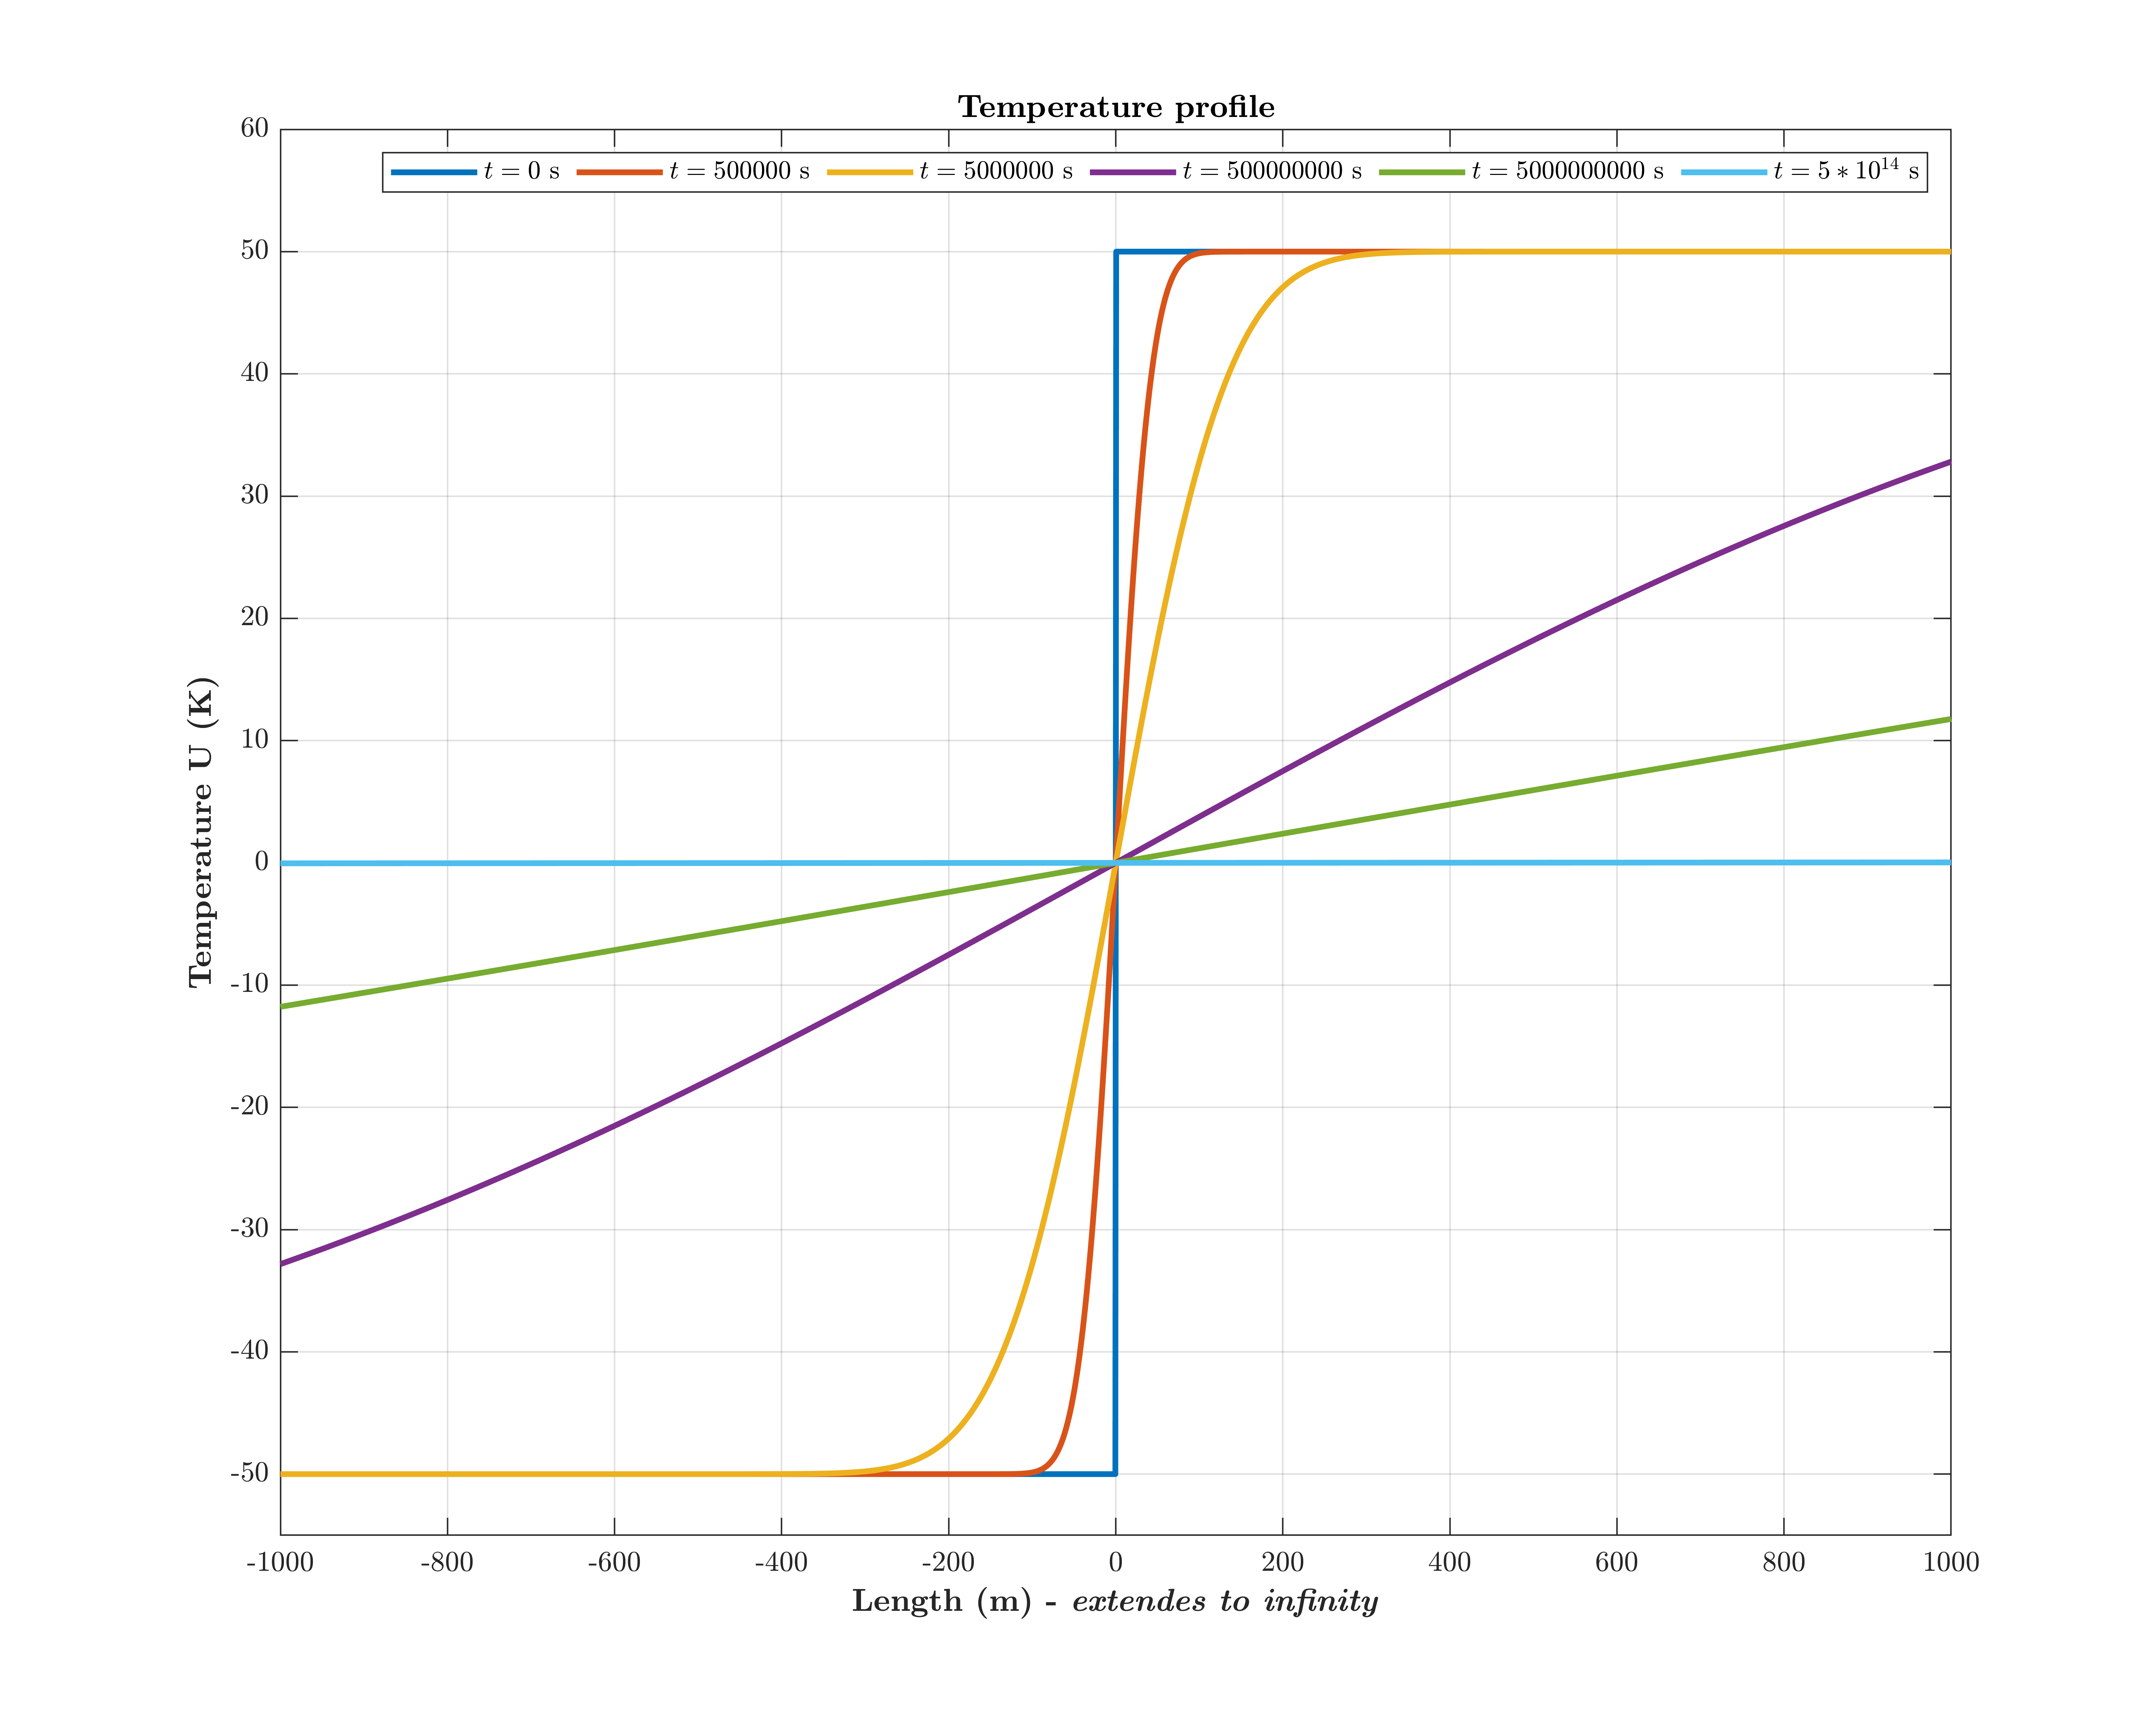
\includegraphics[width=0.8\textwidth]{Images/Problem_3_b.png}
\end{figure}\\
%3b problem ends
%%%%%%%%%%%%%%%%%%%%%%%%%%%%%%%%%%%%%%%%%%%%%%%%%%%%%%%%%%%%%%%%%%%%%%%%%%%%%%%%%%%%%%%%%%%%%
\newpage
%4th Problem starts
\item 
Solve the one-dimensional heat equation
\[
\quad \frac{\partial u}{\partial t} = \alpha \frac{\partial^2 u}{\partial x^2}, \quad 0 < x < \infty, \, t > 0 \\
\]
in a semi-infinite domain for the following initial and boundary conditions\\
\begin{align*}
u(x,0) &= U_i, \quad 0 < x < \infty \\
u(0,t) &= U_0\\
\end{align*}
\emph{\textbf{Solution:}}\\
Using the method of similarity variables,

Given initial condition,
\[
u(x,0) = U_i
\]

Given boundary condition,
\[
u(0,t) = U_o
\]

Boundary condition at \(x = \infty\),
\[
u(\infty,t) = f(x)|_{{x \to \infty}}
\]

Introducing the similarity variable \(\eta\),
\[
\eta = \frac{x}{\sqrt{\alpha t}}
\]

Non-dimensionalizing,
\[
f(\eta) = T = \frac{u(x,t) - u_o}{u_i - u_o}
\]

Boundary conditions,
\[
T(0,t) = 0
\]
\[
T(\infty,t) = 1
\]

Initial condition,
\[
T(x,0) = 1
\]

Solving for \(T(x,t)\) we get,
\[
T(x,t) = \text{erf}\left(\frac{x}{\sqrt{4 \alpha t}}\right)
\]

Transforming back to \(u(x,t)\),
\[
\boxed{
u(x,t) = u_o + (u_i - u_o) \cdot \text{erf}\left(\frac{x}{\sqrt{4 \alpha t}}\right)
}
\]

The values are assumed for plotting, \\
Thermal diffusivity, $\alpha = 1.115 \times 10^{-3}\, \text{m}^2/\text{s}$ \\
Initial temperature, $U_i = 20\, \text{K}$ \\
Temperature at $t > 0$, $U_0 = 50\, \text{K}$ \\
\newpage
The plot is shown below:\\
\begin{figure}[H]
    \centering
    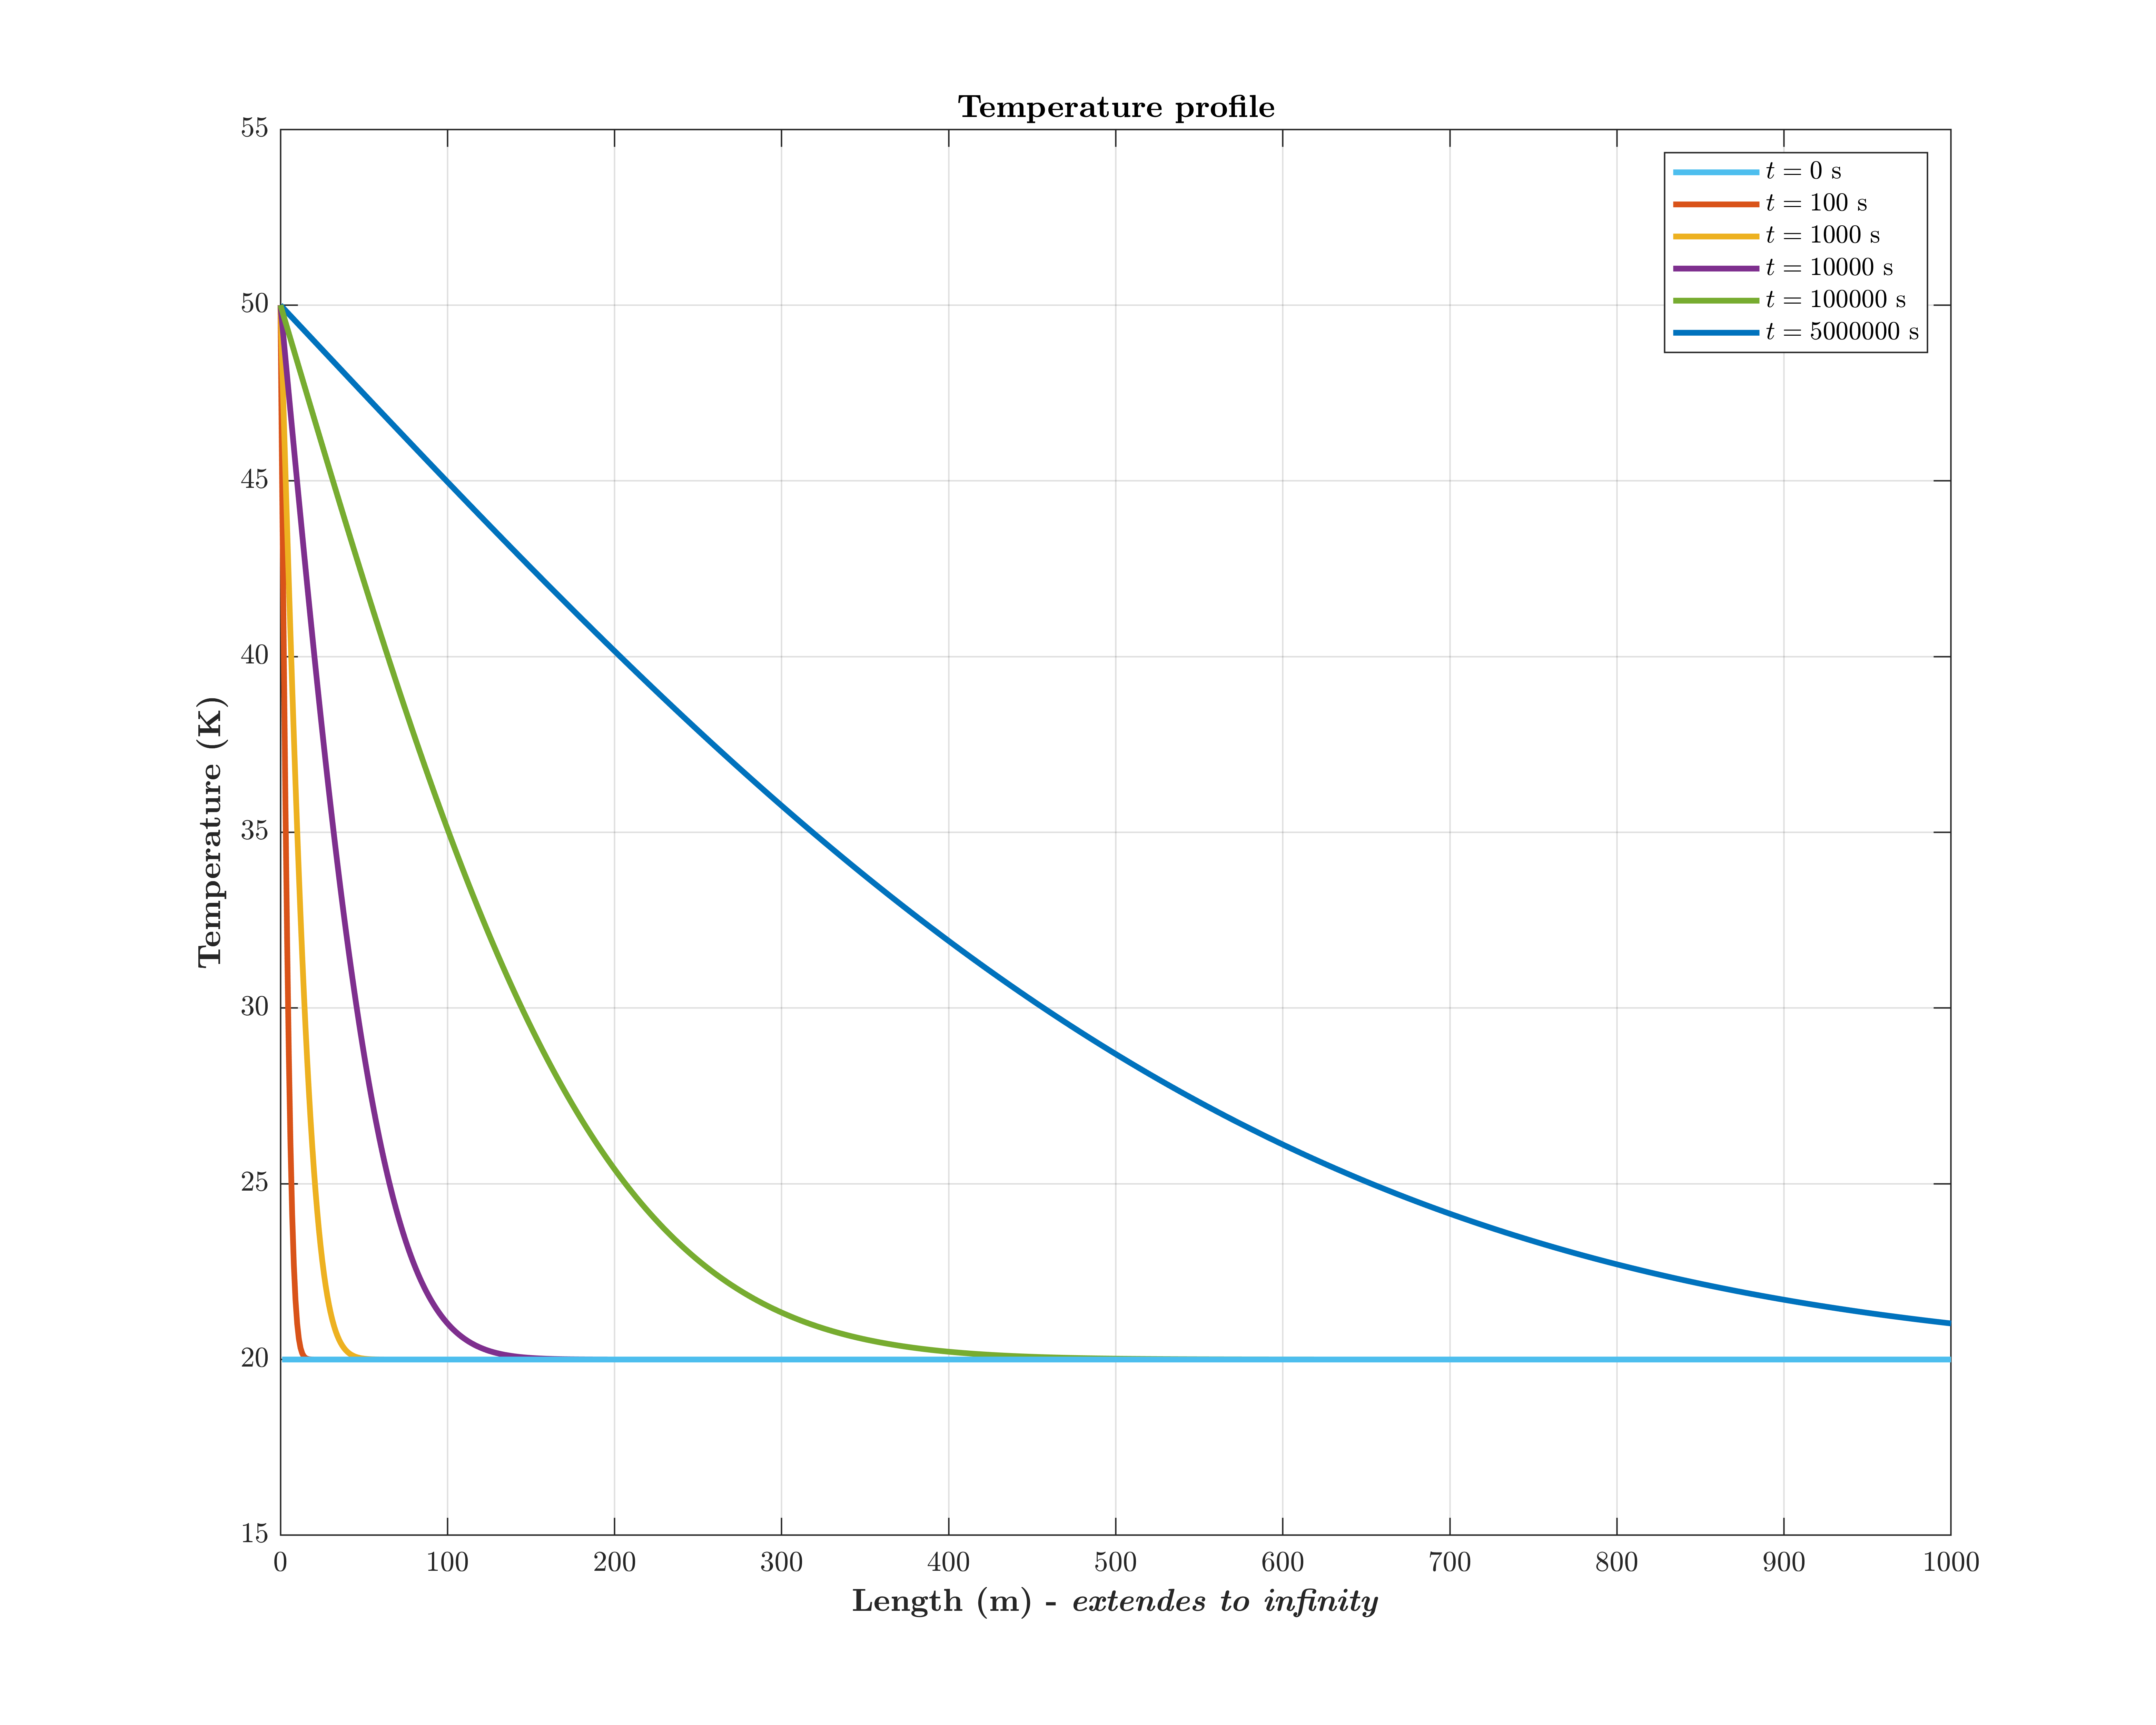
\includegraphics[width=0.8\textwidth]{Images/Problem_4.png}
\end{figure}
%4th Problem ends
\end{enumerate}
\end{document}